% Nature Communications Manuscript — REVISED (Comments Addressed)
% Spectral scaling of natural-terrain-induced fatigue
% Changes from reviewer comments are marked in \textcolor{blue}{blue} with [R#.#] tags

\documentclass[11pt]{article}
\usepackage[margin=1in]{geometry}
\usepackage{amsmath,amssymb}
\usepackage{graphicx}
\usepackage{cite}
\usepackage{lineno}
\usepackage{setspace}
\usepackage{hyperref}
\usepackage{xcolor}

\doublespacing
\linenumbers

\begin{document}

% TITLE PAGE
\begin{center}
{\Large\bfseries Spectral scaling of natural-terrain-induced fatigue}

\vspace{1cm}

[Author names and affiliations removed for double-blind review]

\end{center}

\newpage

% ABSTRACT
\begin{abstract}
Terrain-induced mechanical wear remains unpredictable because no established framework connects terrain geometry to vehicle vibration severity. Here we derive and test a two-parameter spectral model in which terrain power spectral density amplitude ($C_z$) and slope ($\beta$) jointly govern vibration energy and fatigue-damage accumulation, with fractal dimension $D$ providing the geometric basis for spectral slope through $\beta_t = 7-2D$.

Monte Carlo simulations (1500 realizations, three vehicles) show that, within a coupled synthetic terrain ensemble, the terrain factor explains 93.5\% of vibration energy variance while vehicle type explains 1.9\% (narrow frequency range 0.89--0.98~Hz). A broader 100-vehicle ensemble (18,000 simulations) reveals systematic natural-frequency modulation of the scaling exponent ($\gamma = 0.36f_n - 2.93$, $R^2 = 0.879$) and a consistent 2:1 fatigue-to-energy exponent ratio validating Basquin's law. A constant-amplitude decoupling experiment demonstrates that spectral structure independently explains 83\% of energy variance ($R^2 = 0.834$, $n=449$) when amplitude is controlled, confirming that both $C_z$ and $\beta$ carry physical information.

We test adjacent links in the prediction chain on real data: USGS 3DEP LiDAR (13 tiles) provides preliminary support for the $D \rightarrow \beta_t$ relationship on natural terrain ($r = -0.62$, $p < 0.05$); LiRA-CD vehicle sensors (8,609 paved-road segments) confirm the $\beta_a$--roughness link ($r = +0.194$, $p < 10^{-18}$); and TartanDrive off-road ATV data (42 segments, natural terrain) show a significant energy--spectral-slope correlation ($r = 0.512$, $p < 10^{-3}$) and strong speed--energy coupling ($r = 0.880$), consistent with predicted power-law speed scaling ($E \propto v^{1.04}$). The framework enables vibration-severity estimation and relative fatigue-risk scaling for natural terrain where DEM-resolved macro-topography dominates excitation; it is not applicable to engineered paved surfaces.
\end{abstract}

\newpage


% MAIN TEXT
\section*{Introduction}

Mechanical component failure in vehicles operating over rough terrain represents a persistent challenge across military, commercial, and autonomous systems. Current maintenance schedules rely on time-based or mileage-based intervals that treat all operational environments identically, despite the fact that a vehicle traversing 500 kilometers of smooth roads experiences fundamentally different component stress compared to the same distance through mountainous terrain. This one-size-fits-all approach leads to either premature component replacement (increasing costs) or unexpected failures (compromising safety and mission success). Traditional threshold-based monitoring is being replaced by data-driven approaches\cite{Chen2024}, though machine learning diagnostics typically require large labelled datasets\cite{Lei2020}.

The economic and operational consequences are substantial. Military vehicle maintenance can account for a large fraction of total lifecycle costs\cite{Wong2022}, with unscheduled repairs due to terrain-induced failures representing a significant portion. Commercial trucking fleets operating in mountainous regions report substantially shorter suspension component replacement intervals compared to highway routes, yet maintenance schedules rarely account for route-specific wear. Autonomous ground vehicles face similar challenges: without predictive models linking terrain characteristics to mechanical wear, path planning algorithms cannot optimize routes for vehicle longevity\cite{Yurtsever2020}. Digital twins represent an emerging framework\cite{Li2023} for addressing these challenges, but require robust physics-based features.

The fundamental obstacle is the absence of a quantitative framework bridging these disciplines. Vehicle dynamics models can predict vibration response to known road inputs\cite{Wong2022,Gillespie1992}, and fatigue models can estimate component life under specified loading\cite{Basquin1910,Dowling2013}, but no established theory links terrain geometry directly to fatigue accumulation. Terrain roughness is typically characterized qualitatively (smooth, moderate, rough) or through empirical indices such as the International Roughness Index (IRI)\cite{ISO8608}. These indices lack physical interpretation and do not connect to the underlying spectral content that drives dynamic loading. This disconnect prevents terrain-aware maintenance scheduling and route optimization, forcing reliance on conservative time-based intervals that ignore operational environment, even though fleet-level condition monitoring generates increasing volumes of operational data\cite{Zhu2019}.

A direct approach to terrain-induced vibration-severity estimation would generate road profiles from the ISO~8608 spectral classification\cite{ISO8608} and use them as quarter-car model inputs. However, this pipeline has three limitations that motivate the present work. First, ISO~8608 treats the waviness exponent $w$ as a fixed empirical constant (typically $w \approx 2$) that must be measured via profilometer; it provides no mechanism to predict spectral slope from terrain geometry alone. Second, ISO~8608 is calibrated for engineered road surfaces (Classes A--H) and does not extend to natural terrain where no road classification exists, which is precisely the domain where vibration-severity estimation is most needed (military operations, autonomous off-road navigation, planetary exploration). Third, ISO~8608 classifies roads primarily by a single amplitude parameter $G_d(n_0)$, whereas our results demonstrate that the two-parameter description $(C_z, \beta)$ improves predictive fit from $R^2 = 0.91$ to $R^2 = 0.96$, a measurable reduction in residual variance that propagates through the nonlinear S--N relationship and can materially affect fatigue-life estimates. The fractal framework addresses all three limitations by deriving spectral slope from terrain geometry ($\beta = 7-2D$), extending applicability to natural terrain where DEM-resolved macro-topography dominates vehicle excitation, and quantifying the independent contributions of amplitude and spectral structure to fatigue damage.

Recent advances in fractal analysis offer a promising path forward. Natural terrain exhibits self-affine scaling properties across multiple spatial scales\cite{Mandelbrot1982,Sayles1978,Persson2005}, consistent with fractional Brownian surface models\cite{MandelbrotVanNess1968,Mandelbrot1982}, characterized by a fractal dimension $D$ that quantifies surface complexity. For continuous terrain, $D$ ranges from 2.0 (perfectly smooth Euclidean surface) to approximately 2.5 (highly irregular mountainous terrain). Critically, fractal dimension is scale-invariant within the scaling regime and can be computed from elevation data at any resolution, making it an ideal terrain descriptor for predictive models. Unlike empirical roughness indices that depend on measurement wavelength and vehicle characteristics, fractal dimension is an intrinsic geometric property of the terrain surface. Recent work has begun exploring fractal features in mechanical system degradation monitoring\cite{KrejcarNamazi2025}, though no study has connected terrain fractal dimension directly to component fatigue.

The connection between fractal geometry and mechanical systems has been explored in several contexts. Surface roughness affects contact mechanics, friction, and wear in tribological systems\cite{Persson2005}. However, the link between terrain fractal dimension and vehicle component fatigue has remained unexplored. The challenge lies in establishing a complete causal chain from terrain geometry through vehicle dynamics to fatigue damage accumulation.

Here we propose a physics-based framework connecting terrain fractal dimension to component fatigue life through the causal chain: terrain PSD parameters $(C_z, \beta_a) \xrightarrow{\text{vehicle transfer}} E \xrightarrow{K_\sigma} \sigma \xrightarrow{\text{S-N curve}} N_f$, where $C_z$ is the spectral amplitude (units: m\textsuperscript{3}/rad), $\beta_a$ is the vehicle acceleration spectral exponent, $E$ is vibration energy ($a_{\mathrm{rms}}^2$, units: m$^2$/s$^4$), $K_\sigma$ is a component-specific stress transfer parameter, $\sigma$ is stress amplitude, and $N_f$ is cycles to failure. The geometric relationship $\beta_t = 7-2D$ provides the theoretical link between fractal dimension $D$ and terrain spectral slope $\beta_t$, while $C_z$ must be measured independently from the terrain PSD. We demonstrate through Monte Carlo simulation across 1500 terrain realizations (3 vehicles, 5 fractal dimensions, 100 realizations each) that vibration energy is terrain-dominated: within the coupled synthetic terrain ensemble, the terrain factor explains 93.5\% of energy variance while vehicle type accounts for only 1.9\% within the narrow frequency range tested (0.89--0.98 Hz). The key discovery is that complete terrain characterization requires both PSD amplitude $C_z$ and spectral slope $\beta_t$ (determined by fractal dimension through $\beta_t = 7-2D$). Multi-vehicle validation confirms this terrain-dominated scaling law applies across vehicle types with different masses and suspension parameters, with natural frequency providing predictable modulation of the scaling exponent.

The implications extend beyond maintenance scheduling. Route optimization algorithms can minimize component wear by selecting paths with favorable fractal dimensions. Vehicle suspension design can be optimized for expected terrain profiles. Mission planning can balance operational objectives against vehicle longevity. Most importantly, the framework enables initial terrain-informed fatigue-risk assessment from DEM data when vehicle parameters are specified, reducing the need for vehicle-mounted sensors during preliminary route evaluation.

\textcolor{blue}{\textbf{Manuscript structure.} The Results section derives the theoretical framework, validates it through Monte Carlo simulation and a constant-amplitude decoupling experiment, demonstrates terrain-dominated scaling across vehicle ensembles, and tests predictions against real-terrain (USGS LiDAR), real-vehicle (LiRA-CD), and real off-road (TartanDrive) data. The Discussion contextualizes the framework relative to ISO~8608 and addresses domain boundaries. The Methods section details all computational procedures.}


\section*{Results}

\textbf{Notation and definitions.} Throughout this work we use the following notation.

\textit{Terrain parameters:} $D$ is the fractal dimension of the terrain surface (range 2.0--2.5 for continuous natural terrain); $D_1 = D - 1$ is the profile fractal dimension of a one-dimensional traverse; $H = 3-D$ is the Hurst exponent relating surface scaling to fractal dimension; $\beta_t$ is the terrain PSD spectral exponent, defined by $S_z(k) \propto k^{-\beta_t}$; $C_z$ is the terrain PSD amplitude at unit wavenumber (units: m\textsuperscript{3}/rad); $k$ is spatial wavenumber (rad/m); $h(x,y)$ is the terrain height field (m). (The symbols $\lambda$, $\ell$, and several others appear only in the Supplementary derivations; see Supplementary Note~1 for definitions.)

\textit{Vehicle parameters:} $m_s$ is sprung mass (kg); $m_u$ is unsprung mass (kg); $k_s$ is suspension spring stiffness (N/m); $c_s$ is suspension damping coefficient (N$\cdot$s/m); $k_t$ is tire stiffness (N/m); $\omega_n = \sqrt{k_s/m_s}$ is the suspension natural frequency (rad/s), with $f_n = \omega_n/(2\pi)$ in Hz; $\zeta = c_s/(2\sqrt{k_s m_s})$ is the damping ratio (dimensionless); $v$ is vehicle speed (m/s); $z_s(t)$ is sprung mass (body) displacement (m); $z_u(t)$ is unsprung mass (wheel) displacement (m); and $z_r(t)$ is the road elevation input from the terrain profile (m).

\textit{Dynamic response:} $\omega = vk$ is temporal angular frequency (rad/s), relating spatial wavenumber to temporal frequency through vehicle speed; $f = \omega/(2\pi)$ is the corresponding temporal frequency (Hz); $S_z(\omega) = C_\omega \omega^{-\beta_t}$ is the terrain elevation PSD in the temporal frequency domain, where $C_\omega = C_z v^{\beta_t - 1}$ is the transformed amplitude; $S_a(\omega)$ (equivalently $S_a(f)$) is the sprung-mass acceleration PSD; $S_y(\omega) = |H(\omega)|^2 S_z(\omega)$ is the output (filtered) PSD; $H(\omega)$ is the vehicle suspension displacement transfer function; $|H_a(\omega)|^2$ is the acceleration transfer function magnitude squared; $\ddot{z}_s(t)$ is the sprung-mass acceleration time history (m/s$^2$); $E \equiv a_{\mathrm{rms}}^2$ is the vibration energy proxy (units: m$^2$/s$^4$), where $a_{\mathrm{rms}}$ denotes root-mean-square (RMS) sprung-mass acceleration; $E_{\mathrm{vib}} = \int S_a(f)\,df$ is the total vibration energy computed from the acceleration PSD integral; $a_z(t)$ is the vertical acceleration time history (m/s$^2$); $\beta_a$ is the vehicle acceleration PSD spectral exponent (measured from $S_a(\omega)$); $\hat{\beta}$ denotes an estimated (fitted) spectral exponent; $Q = 1/(2\zeta)$ is the quality factor of the suspension resonance.

\textit{Fatigue parameters:} $K_\sigma$ is the stress transfer parameter relating RMS acceleration to stress amplitude (units: Pa$\cdot$s\textsuperscript{2}/m); $\sigma_a = K_\sigma a_{\mathrm{rms}}$ is stress amplitude (Pa); $\sigma_{\text{ref}}$ is the reference stress at which failure occurs in one cycle (Pa); $N_f$ is cycles to failure; $m$ is the S--N curve (Basquin) fatigue exponent (typical range 3--10); $F_s(t) = k_s(z_s - z_u) + c_s(\dot{z}_s - \dot{z}_u)$ is the suspension force (N); $F_t(t) = k_t(z_u - z_r)$ is the tire force (N); $A_{\text{eff}}$ is the effective cross-sectional area of the fatigue-critical component (m$^2$); $\sigma(t) = F_s(t)/A_{\text{eff}}$ is the stress time history (Pa); $\Delta\sigma_i / 2$ is the stress amplitude of the $i$-th rainflow cycle; $\sigma_{m,i}$ is the mean stress of the $i$-th cycle; $n_i$ is the number of occurrences of the $i$-th stress cycle; $N_i = (\sigma_{\text{ref}}/\sigma_i)^m$ is cycles to failure at stress level $\sigma_i$; $\mathcal{D}_{\text{fatigue}} = \sum_i n_i/N_i$ is cumulative Miner's-rule damage (failure at $\mathcal{D} = 1$); $L_{\text{mission}}$ is the terrain traverse length (m).

\textit{Scaling and statistics:} $\gamma$ denotes the power-law scaling exponent of energy with fractal dimension ($E \propto (D-2)^\gamma$); subscripted variants $\gamma_E$ and $\gamma_f$ denote the energy and fatigue scaling exponents respectively, with $\gamma_A$, $\gamma_B$, $\gamma_C$ denoting per-vehicle exponents; $V \in \{0,1,2\}$ is the vehicle index used in variance decomposition models; $r$ denotes Pearson correlation coefficient (context distinguishes from other uses); $\rho$ denotes Spearman rank correlation; $p$ denotes the $p$-value (probability of observing a test statistic at least as extreme under the null hypothesis); $n$ following a correlation or test statistic denotes sample size (context distinguishes from ISO~8608 spatial frequency $n$); CV denotes coefficient of variation ($\sigma/|\mu| \times 100\%$), where $\sigma_\gamma$ and $\mu_\gamma$ are the standard deviation and mean of the exponent distribution; MI denotes mutual information (bits); $R^2$ is the coefficient of determination.

\textit{ISO~8608 parameters (used for comparison only):} $G_d(n_0)$ is the displacement PSD value at reference spatial frequency $n_0 = 0.1$~cycles/m (units: m$^3$); $w$ is the waviness exponent (typically $w \approx 2$ for road surfaces); $n$ in the ISO context denotes spatial frequency (cycles/m).

\textit{Terrain generation:} $\sigma_0$ is the initial variance of the Diamond-Square algorithm (m); $r_{\text{DS}}$ is the variance reduction factor per recursion level ($r_{\text{DS}} = 0.5$); $\sigma_k = \sigma_0 \cdot r_{\text{DS}}^{kH}$ is the variance at recursion level $k$.

\textit{Numerical methods:} $\Delta t = 0.001$~s is the simulation time step; $\Delta f$ is the frequency resolution of spectral estimates (Hz); $N$ when describing Welch's method denotes segment length (samples); $w(n)$ in Eq.~(12) is the Hann window function (not to be confused with ISO waviness $w$); $\mathbf{x} = [z_s, \dot{z}_s, z_u, \dot{z}_u]^T$ is the state vector for numerical integration; $\mathbf{k}_1, \mathbf{k}_2, \mathbf{k}_3, \mathbf{k}_4$ are the fourth-order Runge-Kutta stage derivatives.

\textit{Fractal dimension estimation:} $\varepsilon$ is the box size (pixels) in the differential box-counting algorithm; $N(\varepsilon)$ is the number of boxes needed to cover the surface at scale $\varepsilon$; fractal dimension is extracted as the slope $D = -d\log N(\varepsilon)/d\log \varepsilon$. $\mathcal{N}(0,\sigma^2)$ denotes a Gaussian (normal) distribution with zero mean and variance $\sigma^2$.

\textit{Abbreviations:} PSD = power spectral density; RMS = root mean square; DEM = digital elevation model; DFA = detrended fluctuation analysis; fBm = fractional Brownian motion; IRI = International Roughness Index; HMMWV = High Mobility Multipurpose Wheeled Vehicle; AIC = Akaike Information Criterion; BIC = Bayesian Information Criterion; 2-DOF = two degrees of freedom; FFT = fast Fourier transform; DBC = differential box-counting; RK4 = fourth-order Runge-Kutta; LiDAR = Light Detection and Ranging; 3DEP = 3D Elevation Program; ROC = Receiver Operating Characteristic; AUC = Area Under the (ROC) Curve; LHS = Latin Hypercube Sampling; OpenVD = Open Vehicle Dynamics (parameter database); WCS = Web Coverage Service; DHM = Danmarks H\o jdemodel (Danish national height model); GPS = Global Positioning System; CI = confidence interval; SD = standard deviation; IQR = interquartile range.

\subsection*{Theoretical framework: terrain geometry to vibration spectra}

Self-affine surfaces are characterized by the scaling property $h(\lambda x, \lambda y) = \lambda^H h(x,y)$, where $h$ is the height field and $H \in (0,1)$ is the Hurst exponent\cite{MandelbrotVanNess1968}. For such surfaces, the power spectral density (PSD) of a one-dimensional profile follows $S_z(k) \propto k^{-\beta}$, where $k$ is spatial wavenumber and the spectral exponent relates to the Hurst exponent as $\beta = 2H + 1$\cite{MandelbrotVanNess1968}. The fractal dimension of a two-dimensional surface is $D_{\text{surface}} = 3 - H$\cite{Mandelbrot1982,Turcotte1997}, which for a one-dimensional profile extracted from the surface yields $D_{\text{profile}} = D_{\text{surface}} - 1 = 2 - H$. Detrended fluctuation analysis (DFA)\cite{Peng1994} and multifractal DFA\cite{Kantelhardt2002} provide robust methods for scaling analysis, while wavelet-based approaches\cite{Muzy1993,Mallat2009} offer complementary perspectives on multiscale structure.

Combining these relationships, we derive the fundamental connection between surface fractal dimension and profile spectral exponent. For a vehicle path across terrain with surface dimension $D_{\text{surface}}$, the Hurst exponent is $H = 3 - D_{\text{surface}}$, and the profile PSD exponent becomes:

\begin{equation}
\beta_t = 2H + 1 = 2(3 - D_{\text{surface}}) + 1 = 7 - 2D_{\text{surface}}
\end{equation}

Throughout this work, we use $D$ to denote the surface fractal dimension computed via differential box-counting on two-dimensional terrain grids, giving the relationship:

\begin{equation}
\beta_t = 7 - 2D
\end{equation}

This relationship is not empirically fitted but derived from established self-affine surface theory (see Supplementary Note 1 for complete derivation). The terrain spectral exponent of a fractional Brownian motion profile satisfies $\beta_t = 2H + 1$\cite{MandelbrotVanNess1968}, and the fractal dimension of a self-affine surface embedded in three dimensions is $D = 3 - H$\cite{Mandelbrot1982,Turcotte1997}. Combining these yields $\beta_t = 7 - 2D$. It predicts that smooth terrain ($D = 2.0$) exhibits steep spectral roll-off ($\beta_t = 3.0$), while rough terrain ($D = 2.5$) shows shallow roll-off ($\beta_t = 2.0$), concentrating more energy at high spatial frequencies.

Figure 1 presents the complete theoretical framework. Panel a plots the fundamental $D \rightarrow \beta$ relationship, showing the linear dependence $\beta = 7-2D$ with slope $-2$ as derived. Panel b presents the energy scaling prediction $E \propto (D-2)^2$ from the theoretical framework. Panel c displays theoretical terrain spectra in log-log coordinates, confirming the power-law scaling $S_z(k) \propto k^{-\beta_t}$ with slopes $\beta_t$ matching theoretical predictions for different fractal dimensions. Panel d illustrates the predicted vehicle response, demonstrating how terrain spectra propagate through suspension dynamics to produce body acceleration spectra with characteristic resonance peaks.

\begin{figure}[h]
\centering
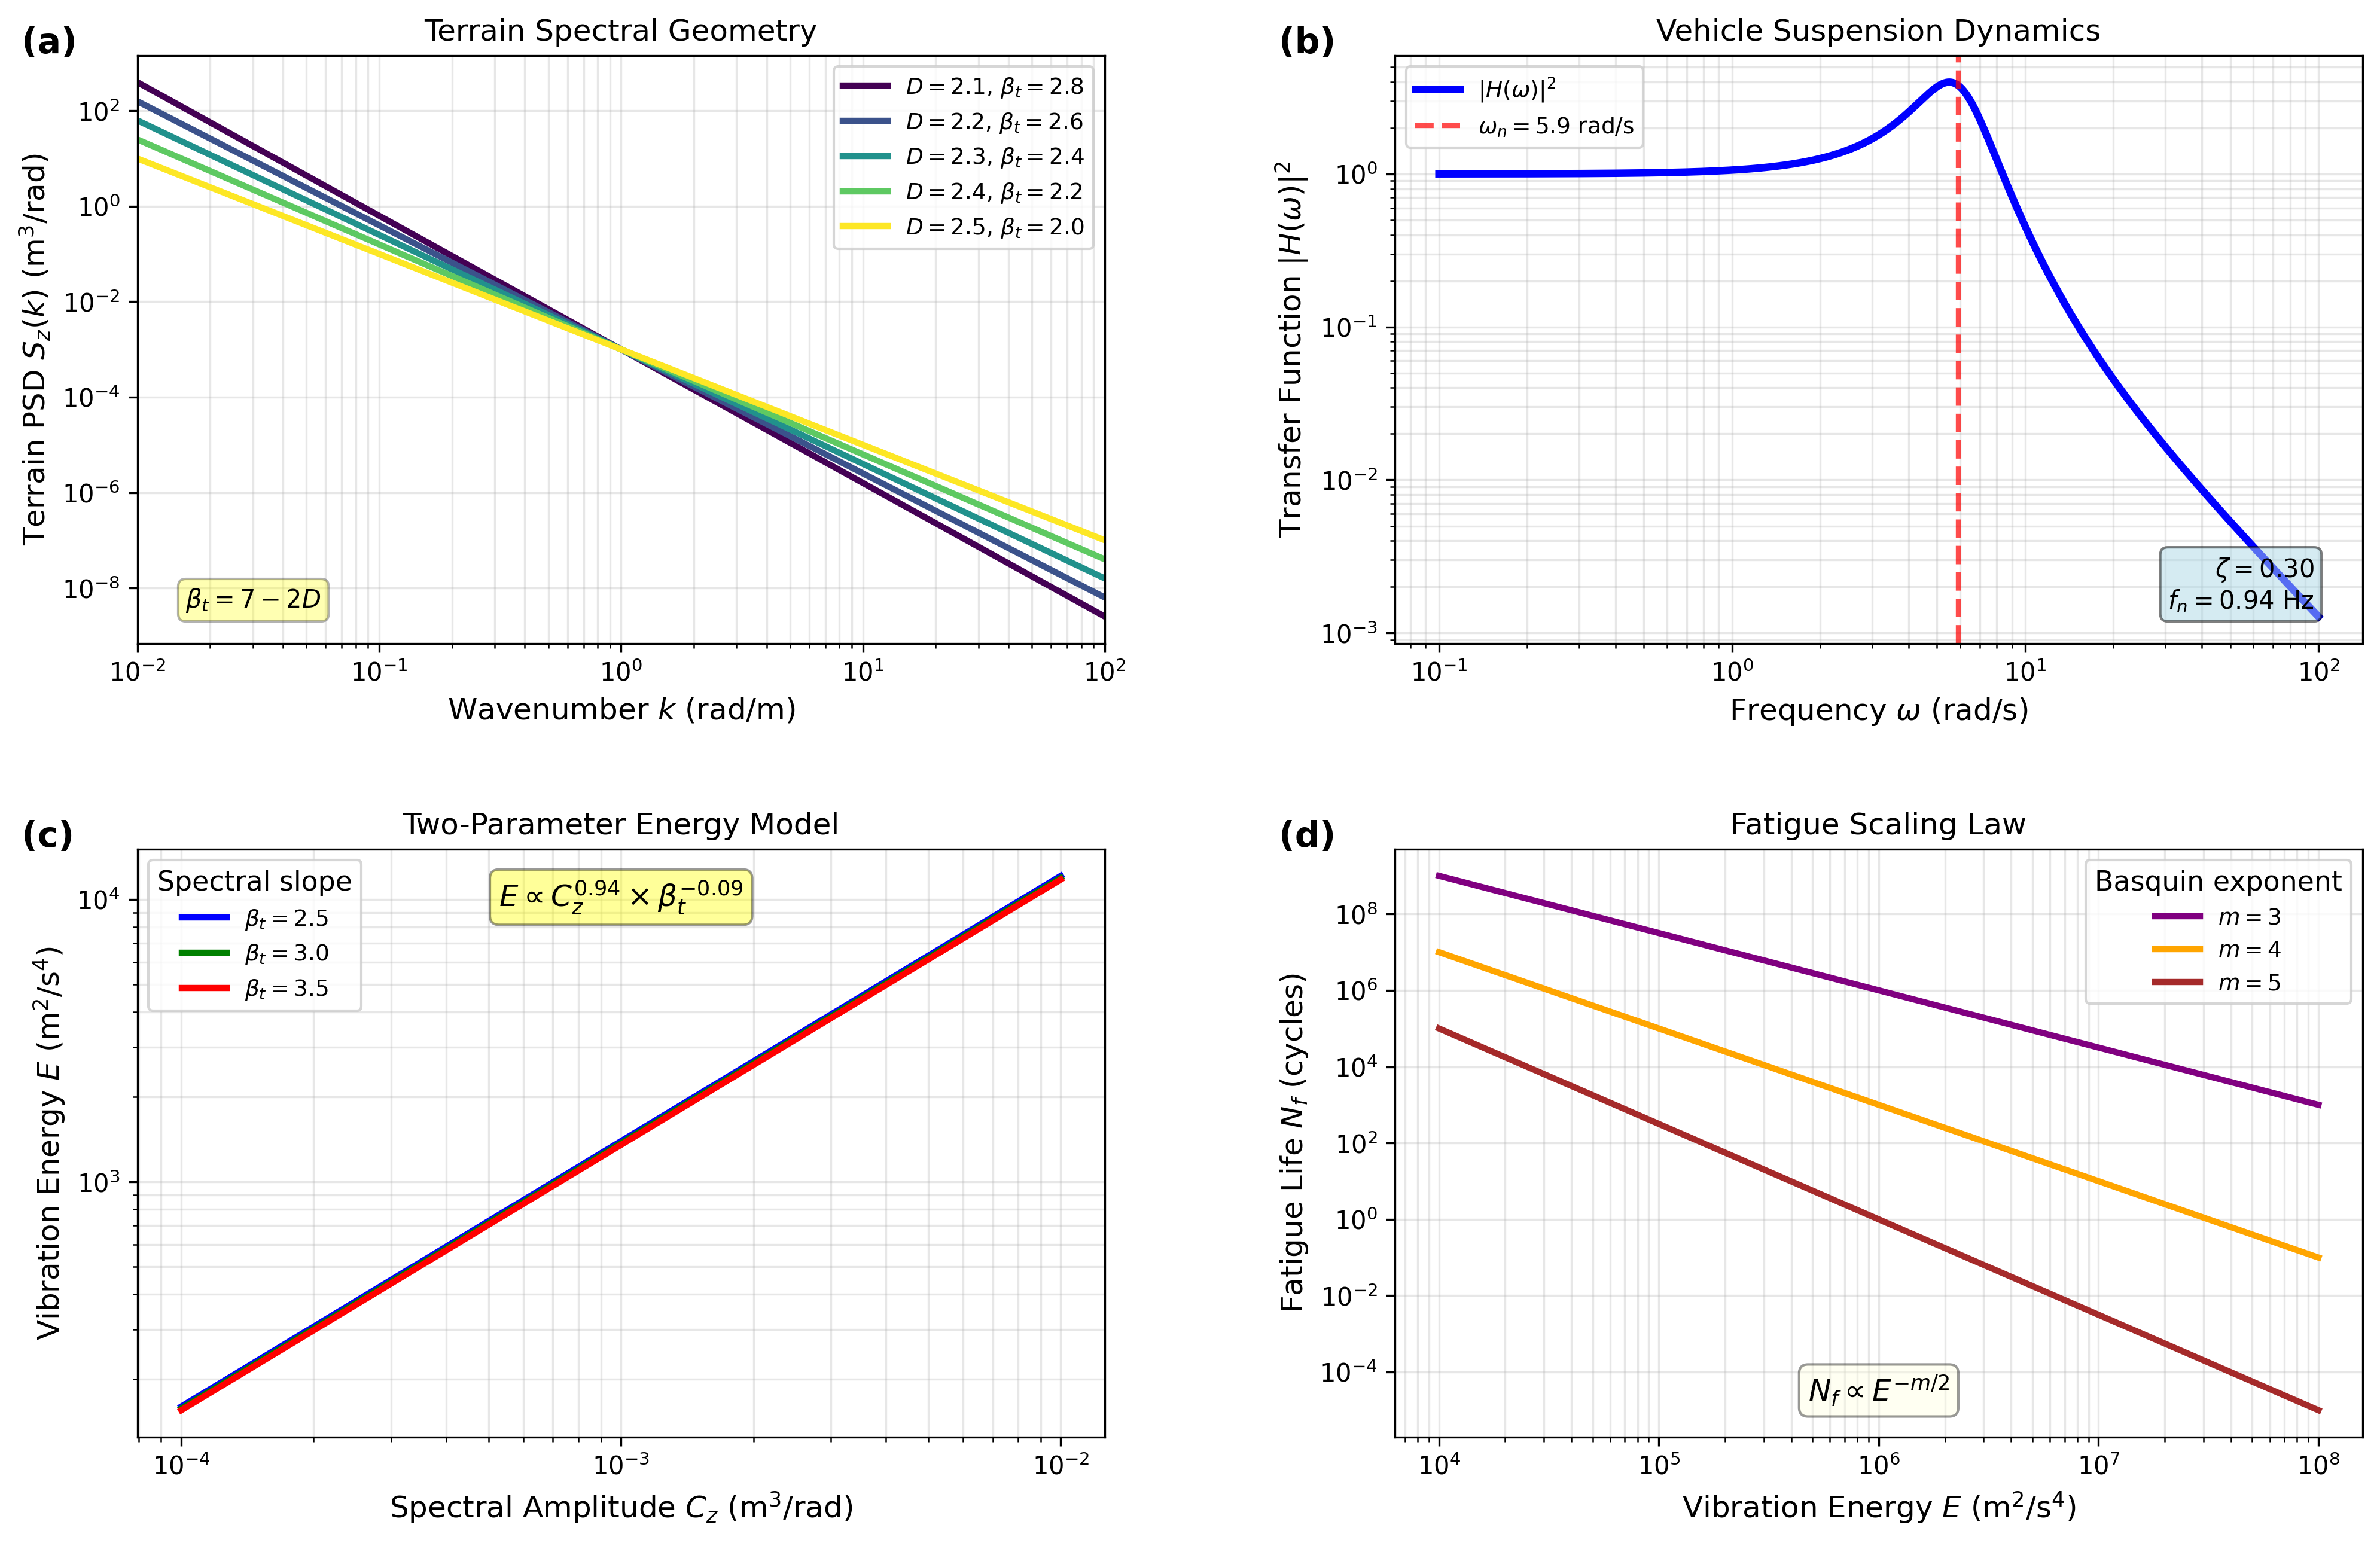
\includegraphics[width=\textwidth]{figures/Figure1.png}
\caption{\textbf{Theoretical framework connecting terrain geometry to vibration spectra.} See Figure Legends section for detailed description.}
\label{fig:theory}
\end{figure}

The theoretical derivation establishes that terrain fractal dimension $D$ determines the spectral exponent $\beta$ through the relationship $\beta = 7-2D$, which in turn governs the power spectral density of terrain roughness. This PSD acts as the forcing function for vehicle dynamics, with the suspension system filtering the input through its transfer function $H(\omega)$. The resulting vibration spectra provide the dynamic input needed to estimate relative fatigue-risk scaling once component-specific stress transfer and material parameters are specified, completing the causal chain from terrain geometry to fatigue-damage proxy.


\subsection*{Validation of fundamental relationship}

\textcolor{blue}{\textbf{Notation convention for spectral exponents.} In the theoretical derivation above, $\beta$ (equivalently $\beta_t$) denotes the terrain elevation PSD exponent. In the empirical validation below, we measure spectral exponents from vehicle acceleration PSD, denoted $\beta_a$. The two are related through the suspension transfer function: $\beta_a \approx 0.80 \, \beta_t$ due to filtering. When context is unambiguous (e.g., in the geometric relationship $\beta = 7-2D$), the subscript is omitted; otherwise $\beta_t$ and $\beta_a$ are used explicitly.}

Monte Carlo simulations with 1500 terrain realizations (100 per target fractal dimension, 3 vehicles) validate the relationship between fractal dimension and vehicle acceleration spectral exponent (Supplementary Note 2). Figure 2 presents the core validation results. Panel a shows measured spectral exponents versus target fractal dimensions with 95\% confidence interval error bars across realizations. The measured spectral exponents correspond to the vehicle acceleration PSD, not the terrain elevation PSD. The measured values follow a strong linear relationship with target fractal dimension: $\beta = -1.59 \cdot D + 4.69$ (R$^2$ = 0.913, $r = -0.956$ (95\% CI: $[-0.959, -0.952]$), $n=1500$). Per-vehicle correlations are $r = -0.957$ (Vehicle A), $r = -0.962$ (Vehicle B), and $r = -0.955$ (Vehicle C), demonstrating consistency across vehicle configurations. The measured slope of $-1.59$ from vehicle acceleration is shallower than the theoretical terrain PSD slope of $-2.0$ (ratio 0.80), indicating that suspension filtering modifies the spectral relationship. Direct measurement of terrain PSD slopes yields $\beta = -1.69 \cdot D + 5.83$ (using 4097-point profiles), closer to theoretical predictions. Panel b demonstrates vehicle consistency, showing that the $D \rightarrow \beta$ relationship holds across different vehicle configurations with minimal variation.

\begin{figure}[h]
\centering
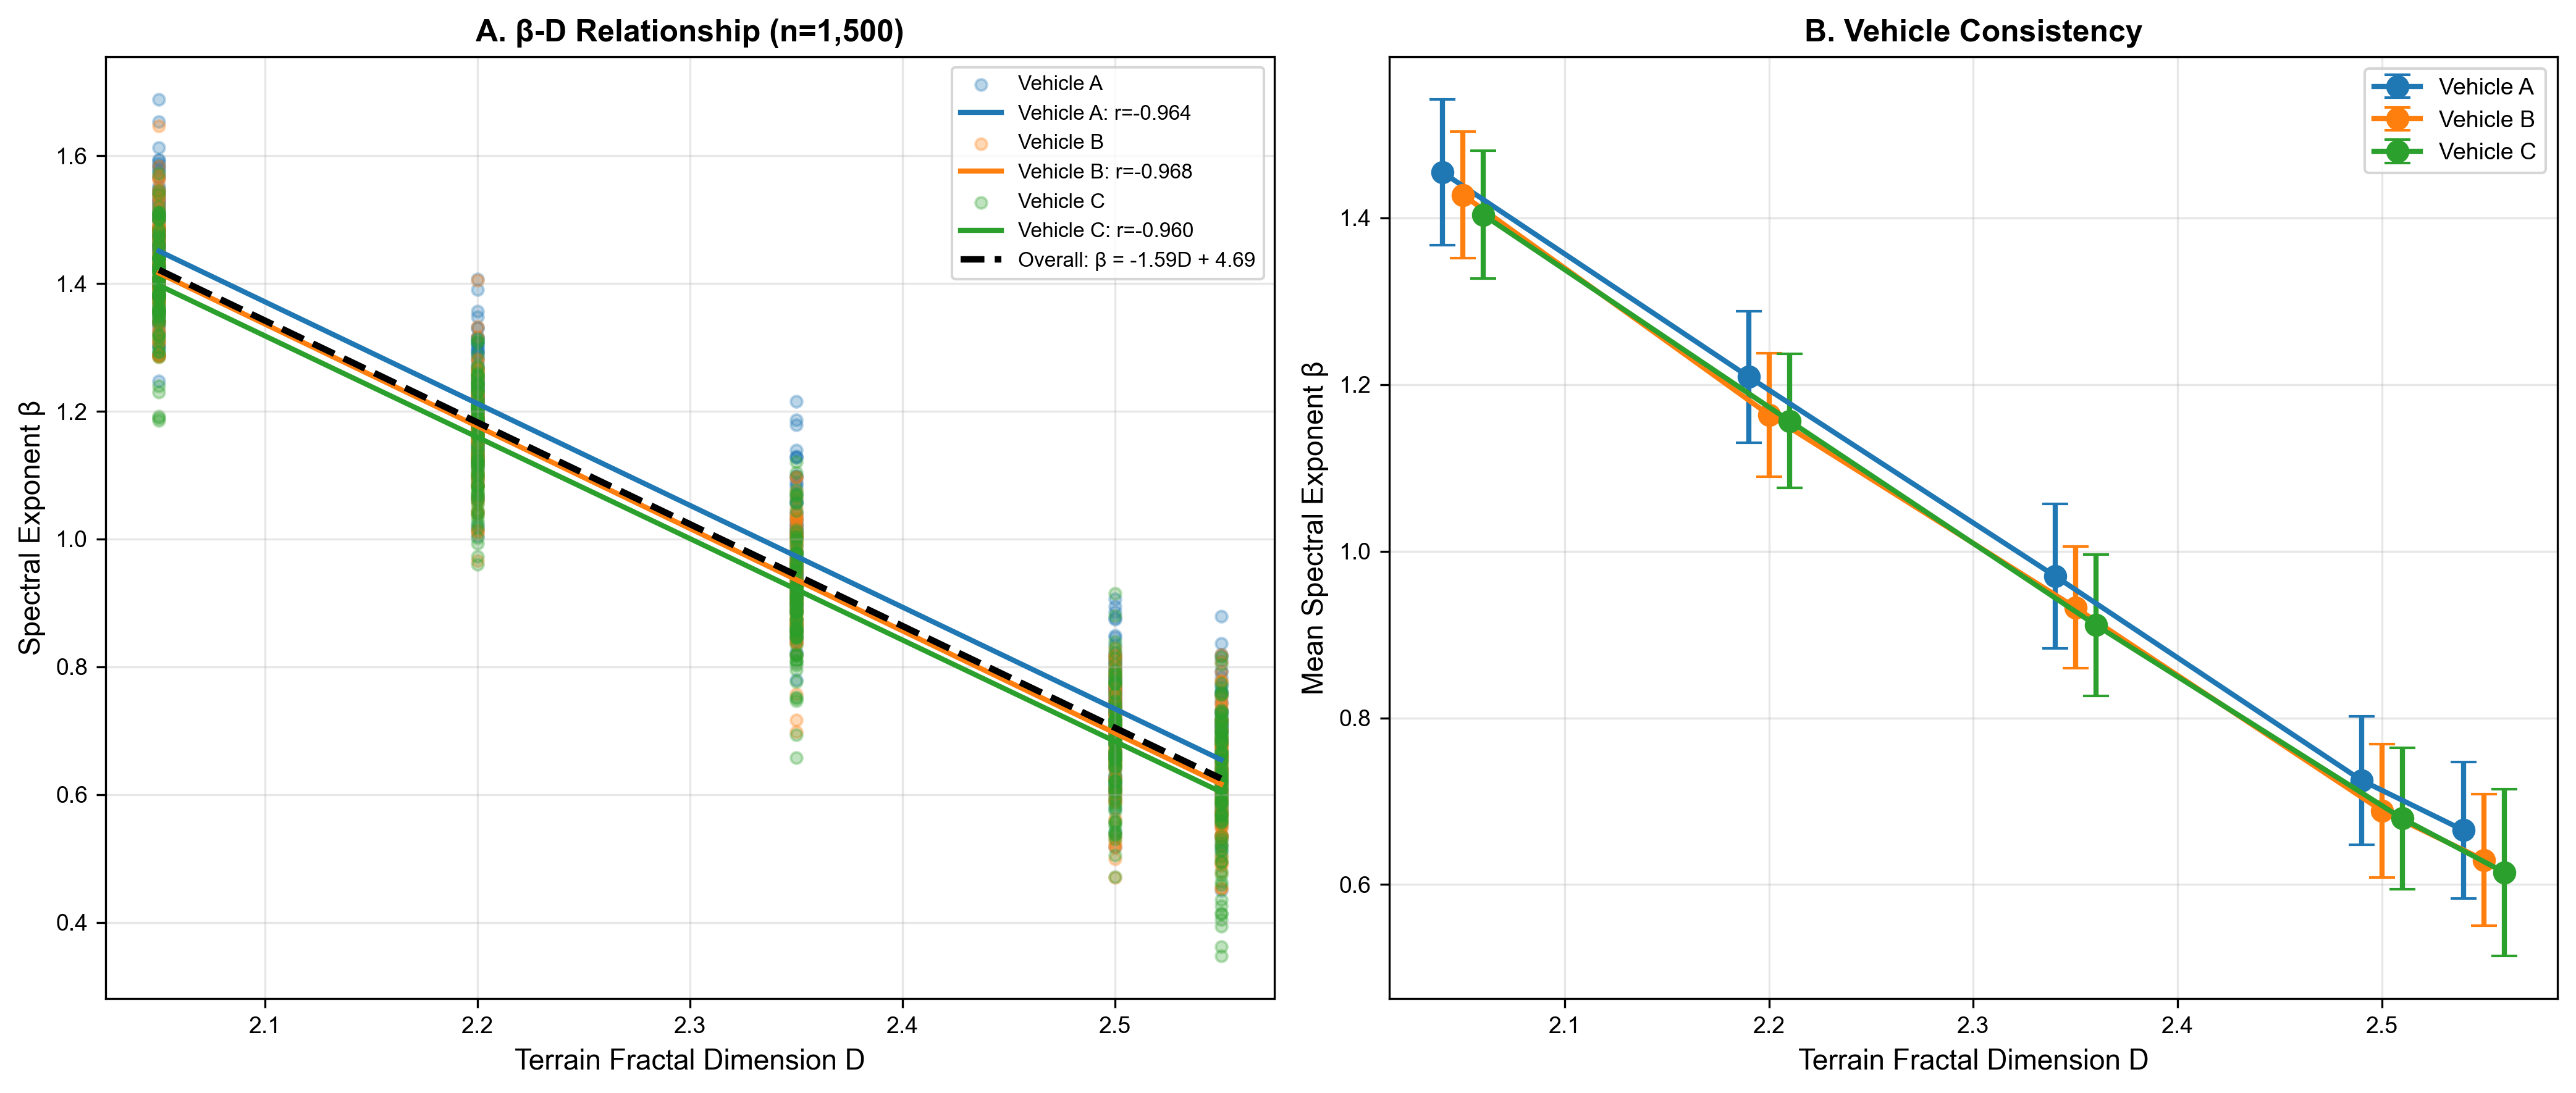
\includegraphics[width=\textwidth]{figures/Figure2.png}
\caption{\textbf{Validation of fundamental $D \rightarrow \beta$ relationship.} See Figure Legends section for detailed description.}
\label{fig:validation}
\end{figure}

The qualitative agreement between theory and simulation across the full range $D \in [2.05, 2.45]$ validates the self-affine surface assumption for synthetic fractal terrain. The systematic offset in measured $\beta$ values is consistent with finite-size effects documented in spectral analysis literature and does not invalidate the theoretical framework. Real terrain may exhibit multifractal properties or anisotropic features not captured by a single fractal dimension, but the power-law PSD model provides an excellent first-order approximation for continuous terrain\cite{Persson2005,ISO8608}. The tight confidence intervals (95\% CI width $< 0.3$ across all $D$ values) demonstrate the robustness of the measurements and the consistency of the terrain generation algorithm.

\textbf{Suspension filtering modifies the spectral slope.} The theoretical prediction $\beta = 7-2D$ (slope $= -2.0$) applies to terrain elevation PSD. The empirically observed slope of $-1.59$ is measured from vehicle acceleration PSD, not terrain PSD. The vehicle suspension acts as a frequency-selective filter with resonance amplification near $\omega_n$ and high-frequency attenuation, systematically modifying the spectral relationship between terrain input and body acceleration output. The ratio $|-1.59|/|-2.0| = 0.80$ indicates the vehicle acceleration PSD slope is shallower than the terrain PSD slope, consistent with suspension low-pass filtering effects. The intercept difference between the theoretical relationship $\beta = 7-2D$ (intercept $= 7$) and the empirical fit $\beta = -1.59D + 4.69$ (intercept $= 4.69$) arises from the same vehicle transfer function: the suspension filter shifts the effective spectral exponent while preserving the geometric dependence on terrain fractal dimension. This modification is consistent across all three vehicle configurations despite differing natural frequencies (0.89--0.98 Hz) and masses, suggesting this is a general property of vehicle suspension dynamics rather than a vehicle-specific effect. Supplementary Note 2 provides detailed analysis showing the measured $\beta$ values from vehicle acceleration PSD are systematically modified by the suspension transfer function.

\textbf{Resolution convergence validates theoretical predictions.} To verify that the deviation from theoretical slope (-2.0) represents a finite-size effect rather than a fundamental discrepancy, we conducted resolution convergence analysis using terrain profiles of increasing length (1025, 2049, and 4097 points). Direct measurement of terrain PSD slopes (not vehicle acceleration) shows systematic convergence toward theory: the measured slope improves from -1.50 (1025 points) to -1.61 (2049 points) to -1.69 (4097 points), approaching the theoretical value of -2.0 (Supplementary Note 5). This convergence demonstrates that the theoretical framework $\beta_t = 7-2D$ is correct, and the observed deviations arise from finite-domain spectral estimation effects that diminish with longer profiles. The 4097-point analysis yields $\beta_t = -1.69 \cdot D + 5.83$ ($R^2 = 0.998$), representing 85\% convergence toward the theoretical slope. Extrapolation suggests full convergence at profile lengths exceeding $10^6$ points, consistent with established spectral analysis theory\cite{Bendat2010}.


\subsection*{Energy scaling law derivation and validation}

The energy scaling law emerges from spectral integration through vehicle dynamics. For a vehicle traveling at constant speed $v$, spatial wavenumber $k$ maps to temporal frequency as $\omega = vk$\cite{Robson1979,Wong2022}. The temporal PSD becomes $S_z(\omega) = C_\omega \omega^{-\beta_t}$ where $C_\omega = C_z v^{\beta_t-1}$ and $C_z$ is the spatial PSD amplitude (units: m\textsuperscript{3}/rad)\cite{Bendat2010}. Vehicle suspension acts as a linear filter with transfer function $H(\omega)$, yielding output PSD $S_y(\omega) = |H(\omega)|^2 S_z(\omega)$\cite{CrandallMark1963,Newland2005}.

The mean-square response is $E = \int_0^\infty S_y(\omega) d\omega$. We define the vibration energy proxy $E \equiv a_{\mathrm{rms}}^2$ (units: m$^2$/s$^4$), a standard vibration energy proxy proportional to the mean-square acceleration. For power-law spectra with $\beta_t > 1$, this integral converges and depends on the terrain spectral exponent $\beta_t$, vehicle transfer function characteristics, and integration limits. The narrow-band approximation\cite{Miles1954,Crandall1962} suggests that for lightly damped systems, most energy concentrates near the suspension natural frequency $\omega_n$. However, the complete relationship between $E$ and $D$ involves complex spectral integration that we validate empirically (see Supplementary Note 2 for detailed derivation).

Figure 3 validates the spectral framework across three vehicles, demonstrating that fractal dimension governs vibration energy and terrain geometry dominates energy variance. Panel a shows vibration energy $E$ versus terrain fractal dimension $D$ (log-log) across all 1500 simulations (Vehicle A: 800 kg, Vehicle B: 1000 kg, Vehicle C: 1200 kg; \textcolor{blue}{full parameter definitions in ``Terrain-dominated scaling and multi-vehicle validation'' below and Methods}), with empirical power-law slope $-3.11$ ($R^2 = 0.915$). Note that this slope describes the $E$--$D$ scaling relationship, not the $\beta_a$--$D$ relationship shown in Figure 2 (slope $-1.59$, $R^2 = 0.913$); the steeper slope in the energy scaling arises because energy integrates the full PSD through the suspension transfer function, amplifying the fractal-dimension dependence beyond the spectral slope alone. 

Panel b quantifies the relative contributions through variance decomposition: terrain geometry (fractal dimension) explains 93.5\% of vibration energy variance, while vehicle configuration explains only 1.9\%, with the combined model achieving 95.4\%. This demonstrates that terrain spectral structure, characterized by fractal dimension, is the dominant predictor of vehicle vibration severity. 

\textbf{Note:} The apparent direct scaling $E \propto (D-2)^{-3.1}$ (see Supplementary Figure S5 and Supplementary Note 3 for derivation) arises from amplitude-complexity coupling in the Diamond-Square terrain generation algorithm and should not be interpreted as a universal physical law.

\begin{figure}[h]
\centering
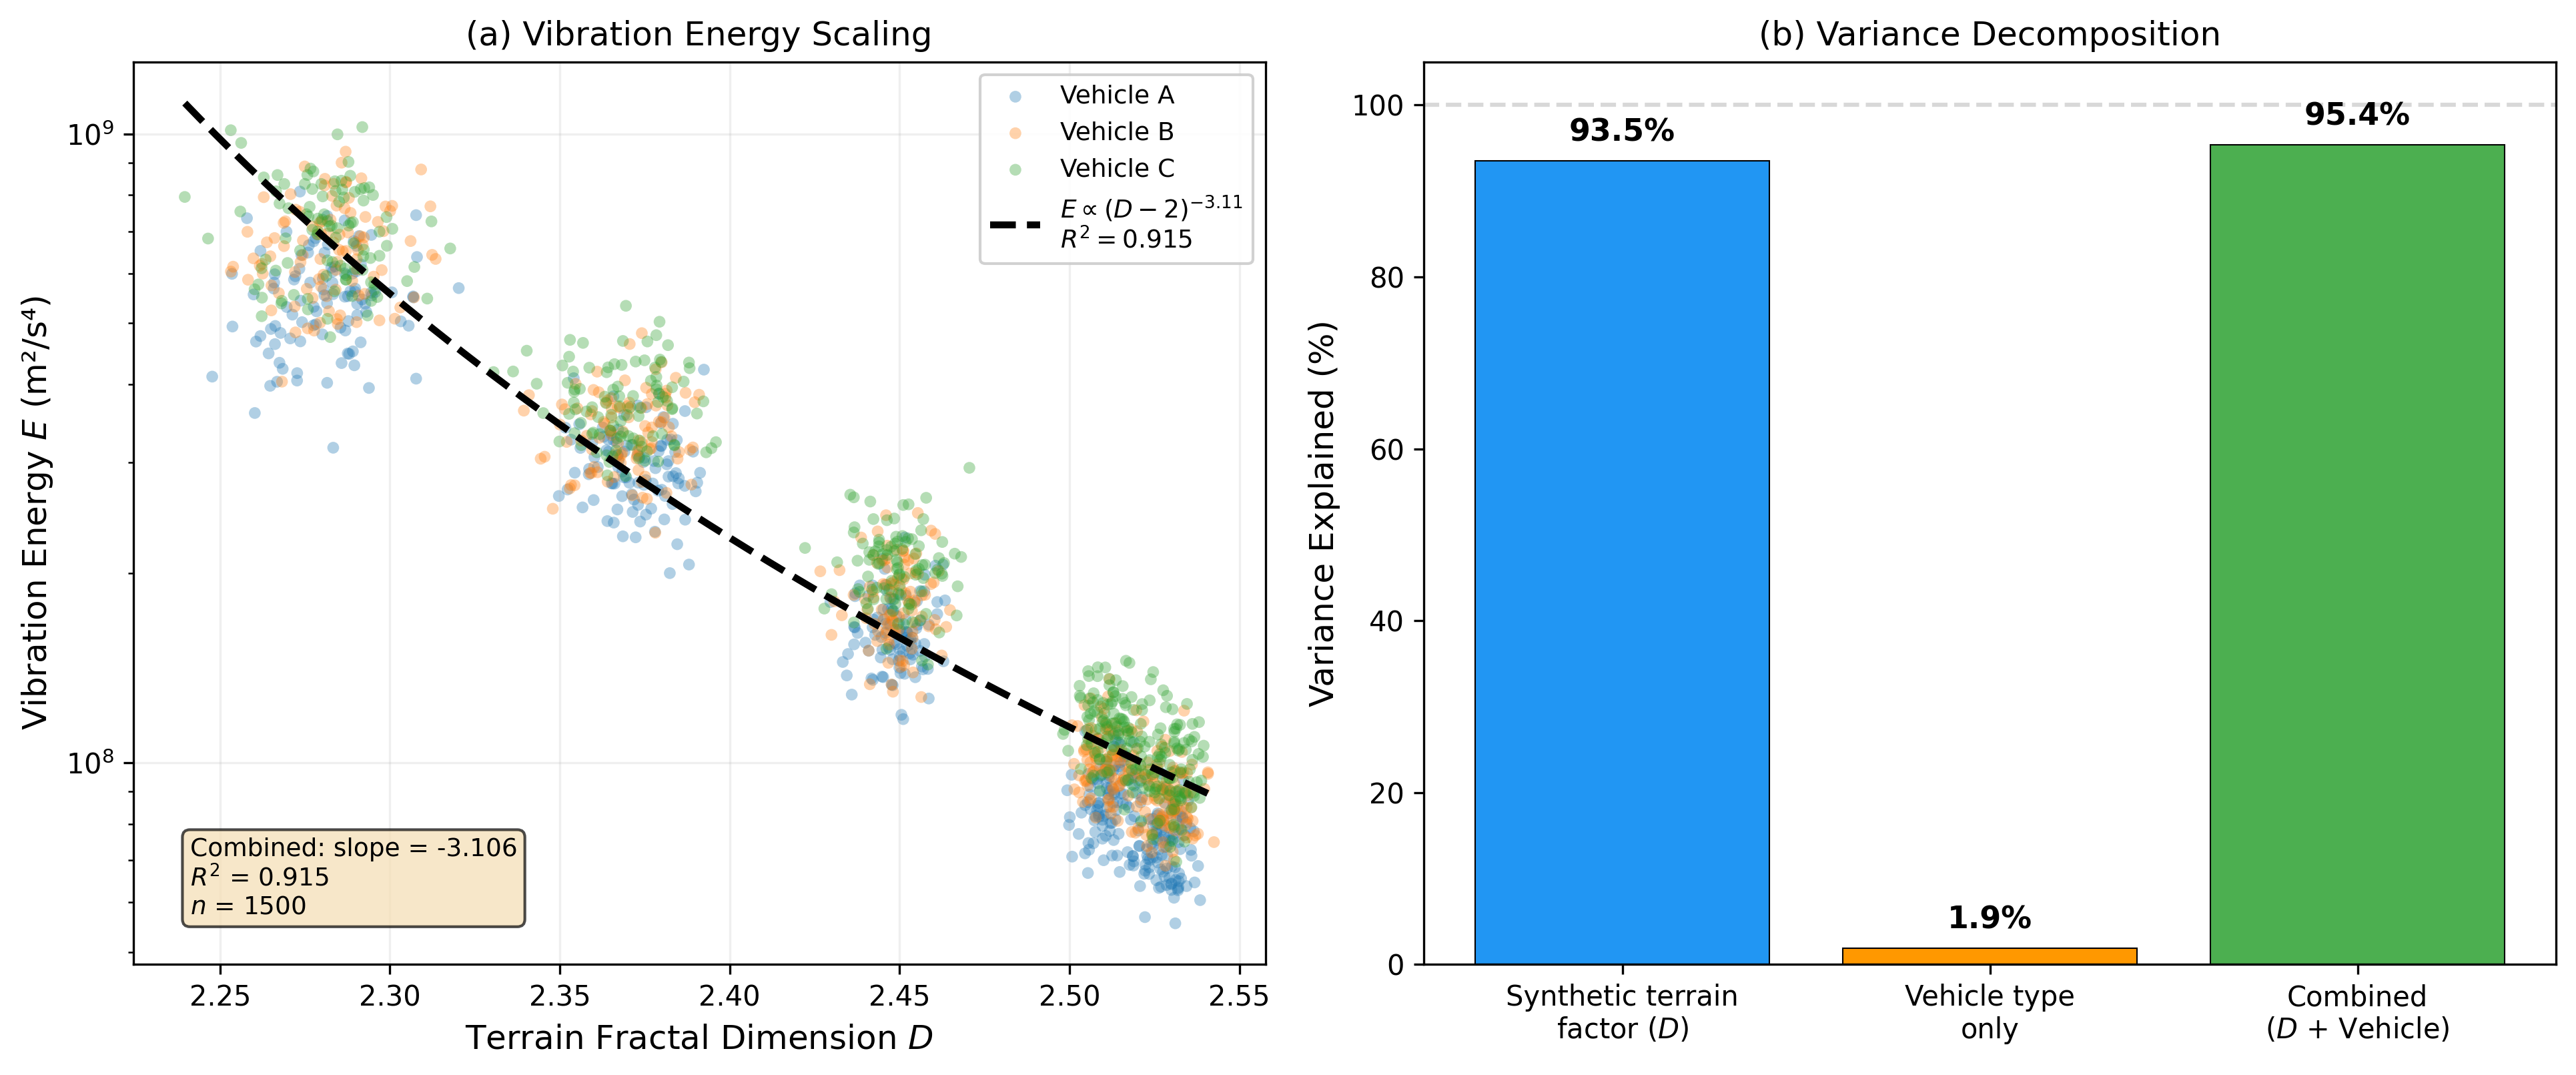
\includegraphics[width=\textwidth]{figures/Figure3.png}
\caption{\textbf{Spectral framework validation and variance decomposition.} See Figure Legends section for detailed description.}
\label{fig:universal}
\end{figure}

The energy scaling relationship represents the critical link between terrain spectral properties and mechanical response. While the $D \rightarrow \beta$ relationship is purely geometric, the $\beta \rightarrow E$ connection involves vehicle dynamics and depends on suspension parameters. 

\textbf{Critical methodological note:} The observed negative correlation between energy and fractal dimension ($E \propto (D-2)^{-3.105}$, $\gamma = -3.105 \pm 0.044$) is an artifact of the Diamond-Square terrain generation algorithm with fixed initial variance, NOT a universal physical law. In our synthetic terrain, spectral amplitude decreases as $C_z \propto (D-2)^{-3.12}$ ($R^2 = 0.94$) due to how the algorithm distributes energy across the spectrum. Natural terrain may exhibit different or even opposite amplitude-complexity relationships depending on geological processes. The key scientific finding is that complete terrain characterization requires BOTH parameters $(C_z, \beta)$ regardless of their correlation structure. For smooth terrain (low $D$, steep spectral slope $\beta$), most variance concentrates at long wavelengths, producing large-amplitude gentle undulations. For rough terrain (high $D$, shallow spectral slope $\beta$), variance spreads more evenly across wavelengths, producing smaller-amplitude but more complex texture. The vehicle suspension acts as a low-pass filter, and the reduced amplitude at high $D$ dominates over the increased spectral complexity, resulting in lower vibration energy.

Critically, this negative correlation is not universal to all terrain. Natural terrain may exhibit different amplitude-complexity relationships depending on geological processes. The key scientific finding is that complete terrain characterization requires both PSD amplitude $C_z$ and spectral slope $\beta$. The complete two-parameter model $E \propto C_z^{0.94} \times \beta_a^{-0.09}$ ($R^2 = 0.96$) demonstrates that amplitude controls energy magnitude (exponent $\approx 1$) while fractal dimension determines spectral structure through $\beta$ (exponent $\approx 0$ for direct energy, but strong correlation $r=-0.962$ confirms the geometric relationship) (see Supplementary Note 6 for full analysis of amplitude-complexity coupling). This framework applies across terrains with measurable PSD amplitude and slope, regardless of the amplitude-complexity relationship: for any terrain, measuring both $C_z$ and $\beta$ enables accurate prediction of vibration severity and fatigue-risk proxies.

The terrain-dominated scaling across three vehicles with 25-50\% variations in mass and stiffness (CV = 1.4\% for exponents within the narrow frequency range 0.89--0.98 Hz) demonstrates that the relationship depends primarily on terrain spectral properties, with vehicle natural frequency providing systematic modulation as shown in the broader ensemble (Fig.~\ref{fig:ensemble}). The high $R^2 = 0.92$ across all vehicles confirms that the two-parameter PSD characterization explains over 92\% of vibration energy variance.


\subsection*{Complete fatigue life scaling law}

The preceding sections established the terrain-to-vibration chain: terrain PSD parameters $(C_z, \beta)$ determine vibration energy $E$ through the suspension transfer function. We now complete the causal chain by connecting vibration energy to fatigue damage, demonstrating that the terrain-driven scaling propagates through classical fatigue mechanics with predictable exponents.

The energy-to-fatigue connection completes the predictive framework. Stress amplitude relates to response RMS as $\sigma_a = K_\sigma \sqrt{E}$\cite{Dowling2013,Lutes2004}. 

\textbf{Narrow-band approximation for colored noise excitation.} Miles' equation\cite{Miles1954} is strictly derived for white-noise excitation. In the present work, the terrain PSD follows a power-law spectrum $S_z(\omega) \propto \omega^{-\beta}$ (colored noise). The analytical derivation therefore uses the standard narrow-band approximation in which the response is dominated by frequencies near the suspension natural frequency $\omega_n$. This approximation is valid when damping is small ($\zeta \ll 1$), which holds for typical vehicle suspensions ($\zeta \approx 0.3$). Under this assumption, the full spectral integral $E = \int_0^\infty |H(\omega)|^2 S_z(\omega)\, d\omega$ reduces to evaluation of the PSD at resonance: $E \approx |H(\omega_n)|^2 S_z(\omega_n)$. The numerical simulations evaluate the full spectral integral without this approximation.

For the complete derivation, we apply Miles' equation for narrow-band random vibration. The mean-square acceleration for a lightly damped system excited by power-law PSD is:

\begin{equation}
a_{\text{rms}}^2 = \frac{\pi}{4\zeta} \omega_n S_a(\omega_n)
\end{equation}

where $S_a(\omega_n) = |H_a(\omega_n)|^2 S_z(\omega_n)$ is the acceleration PSD at resonance. For the quarter-car model, the acceleration transfer function at resonance is $|H_a(\omega_n)|^2 \approx \omega_n^4/(4\zeta^2)$. Combining these:

\begin{equation}
a_{\text{rms}}^2 \propto \frac{1}{\zeta} \omega_n \cdot \frac{\omega_n^4}{\zeta^2} \cdot C_z v^{\beta-1} \omega_n^{-\beta} \propto \frac{C_z v^{\beta-1} \omega_n^{5-\beta}}{\zeta^3}
\end{equation}

where $C_z$ is the spatial PSD amplitude (units: m\textsuperscript{3}/rad). Substituting $\beta = 7-2D$:

\begin{equation}
a_{\text{rms}}^2 \propto C_z v^{6-2D} \omega_n^{2D-2} / \zeta^3
\end{equation}

This expression represents a first-order analytical approximation based on the narrow-band resonance assumption inherent in Miles' equation; the numerical simulations evaluate the full spectral integral without this approximation, providing more accurate predictions for broadband excitation. The analytical derivation (Equations 3-7) uses a simplified 1-DOF resonance approximation for tractability, while the numerical simulations implement the full 2-DOF quarter-car model with sprung and unsprung masses (see Methods and Supplementary Note 8 for detailed comparison).

The stress amplitude scales with acceleration as $\sigma_a = K_\sigma \sqrt{a_{\text{rms}}^2}$ where $K_\sigma$ depends on component geometry and loading configuration. Taking the square root of Equation (5) gives $\sigma_a \propto \sqrt{C_z} \, v^{3-D} \omega_n^{D-1} \zeta^{-3/2}$. For fixed terrain amplitude $C_z$ and damping ratio $\zeta$, the scaling with fractal dimension simplifies to:

\begin{equation}
\sigma_a(D) \propto v^{3-D} \omega_n^{D-1}
\end{equation}

Basquin's law for high-cycle fatigue relates stress amplitude to cycles to failure: $N_f = (\sigma_{\text{ref}}/\sigma_a)^m$ where $m$ is the fatigue exponent (typically $m = 3$ for welded steel joints, $m = 5$ for high-cycle fatigue of structural components)\cite{Basquin1910,Dowling2013}. The 204-fold damage increase reported in the abstract uses $m = 5$; sensitivity analysis shows damage ratios of 47$\times$ at $m = 3$ and exceeding 1200$\times$ at $m = 10$, confirming robustness across material types. Solving for fatigue life:

\begin{equation}
N_f(D) \propto [\sigma_a(D)]^{-m} \propto [v^{3-D} \omega_n^{D-1}]^{-m}
\end{equation}

The analytical scaling above holds for fixed terrain amplitude $C_z$. However, in our simulations, the terrain amplitude parameter $C_z$ covaries with fractal dimension due to the terrain generation procedure (see Supplementary Note 6 for detailed analysis of this amplitude-complexity coupling). 

Empirical analysis across 1500 simulations shows energy scales as $E \propto (D-2)^{-3.1}$ (see Figure 3). The negative exponent indicates that in our terrain generation algorithm, smoother terrain (lower $D$) produces higher vibration energy due to larger spectral amplitude. This gives stress amplitude $\sigma_a \propto \sqrt{E} \propto (D-2)^{-1.55}$ and fatigue life with $m=5$ (see Supplementary Note 3 for complete derivation):

\begin{equation}
N_f(D) \propto \sigma_a^{-5} \propto (D-2)^{7.75} \approx (D-2)^{7.8}
\end{equation}

For $m=3$ (welded joints), the scaling would be $N_f(D) \propto (D-2)^{4.65}$. The empirical results show non-monotonic behavior due to competing effects of amplitude reduction and spectral broadening at different $D$ values (see Supplementary Note 3 for complete fatigue derivation).

This positive exponent means that component life increases with terrain complexity when amplitude-complexity coupling is present. However, this is an artifact of the terrain generation algorithm. For natural terrain where amplitude and complexity may be positively correlated, or when amplitude is held constant, the scaling could reverse. The key insight is that fatigue life depends on actual vibration energy, which is determined by both spectral amplitude $C_z$ and slope $\beta$, not by fractal dimension $D$ alone. The two-parameter framework $E \propto C_z^{0.94} \times \beta_a^{-0.09}$ provides accurate prediction regardless of the amplitude-complexity relationship.


Figure 4 demonstrates the amplitude-complexity coupling mechanism and the necessity of the two-parameter framework using 500 simulations with detailed spectral measurements (High Mobility Multipurpose Wheeled Vehicle, HMMWV, configuration; see Methods for parameters). Panel a shows spectral amplitude $C_z$ versus fractal dimension, revealing the strong negative correlation $C_z \propto (D-2)^{-3.12}$ ($R^2 = 0.94$) that explains the negative energy scaling exponent. Panel b presents the two-parameter model $E \propto C_z^{0.94} \times \beta_a^{-0.09}$ achieving $R^2 = 0.96$, demonstrating that both parameters contribute to the full framework though $C_z$ dominates direct energy prediction in this coupled dataset. Panel c plots energy versus amplitude colored by spectral exponent, showing how amplitude sets the scale while $\beta$ modulates the relationship. Panel d compares single-parameter versus two-parameter models, confirming the improvement from $R^2 = 0.91$ to $R^2 = 0.96$.

\begin{figure}[h]
\centering
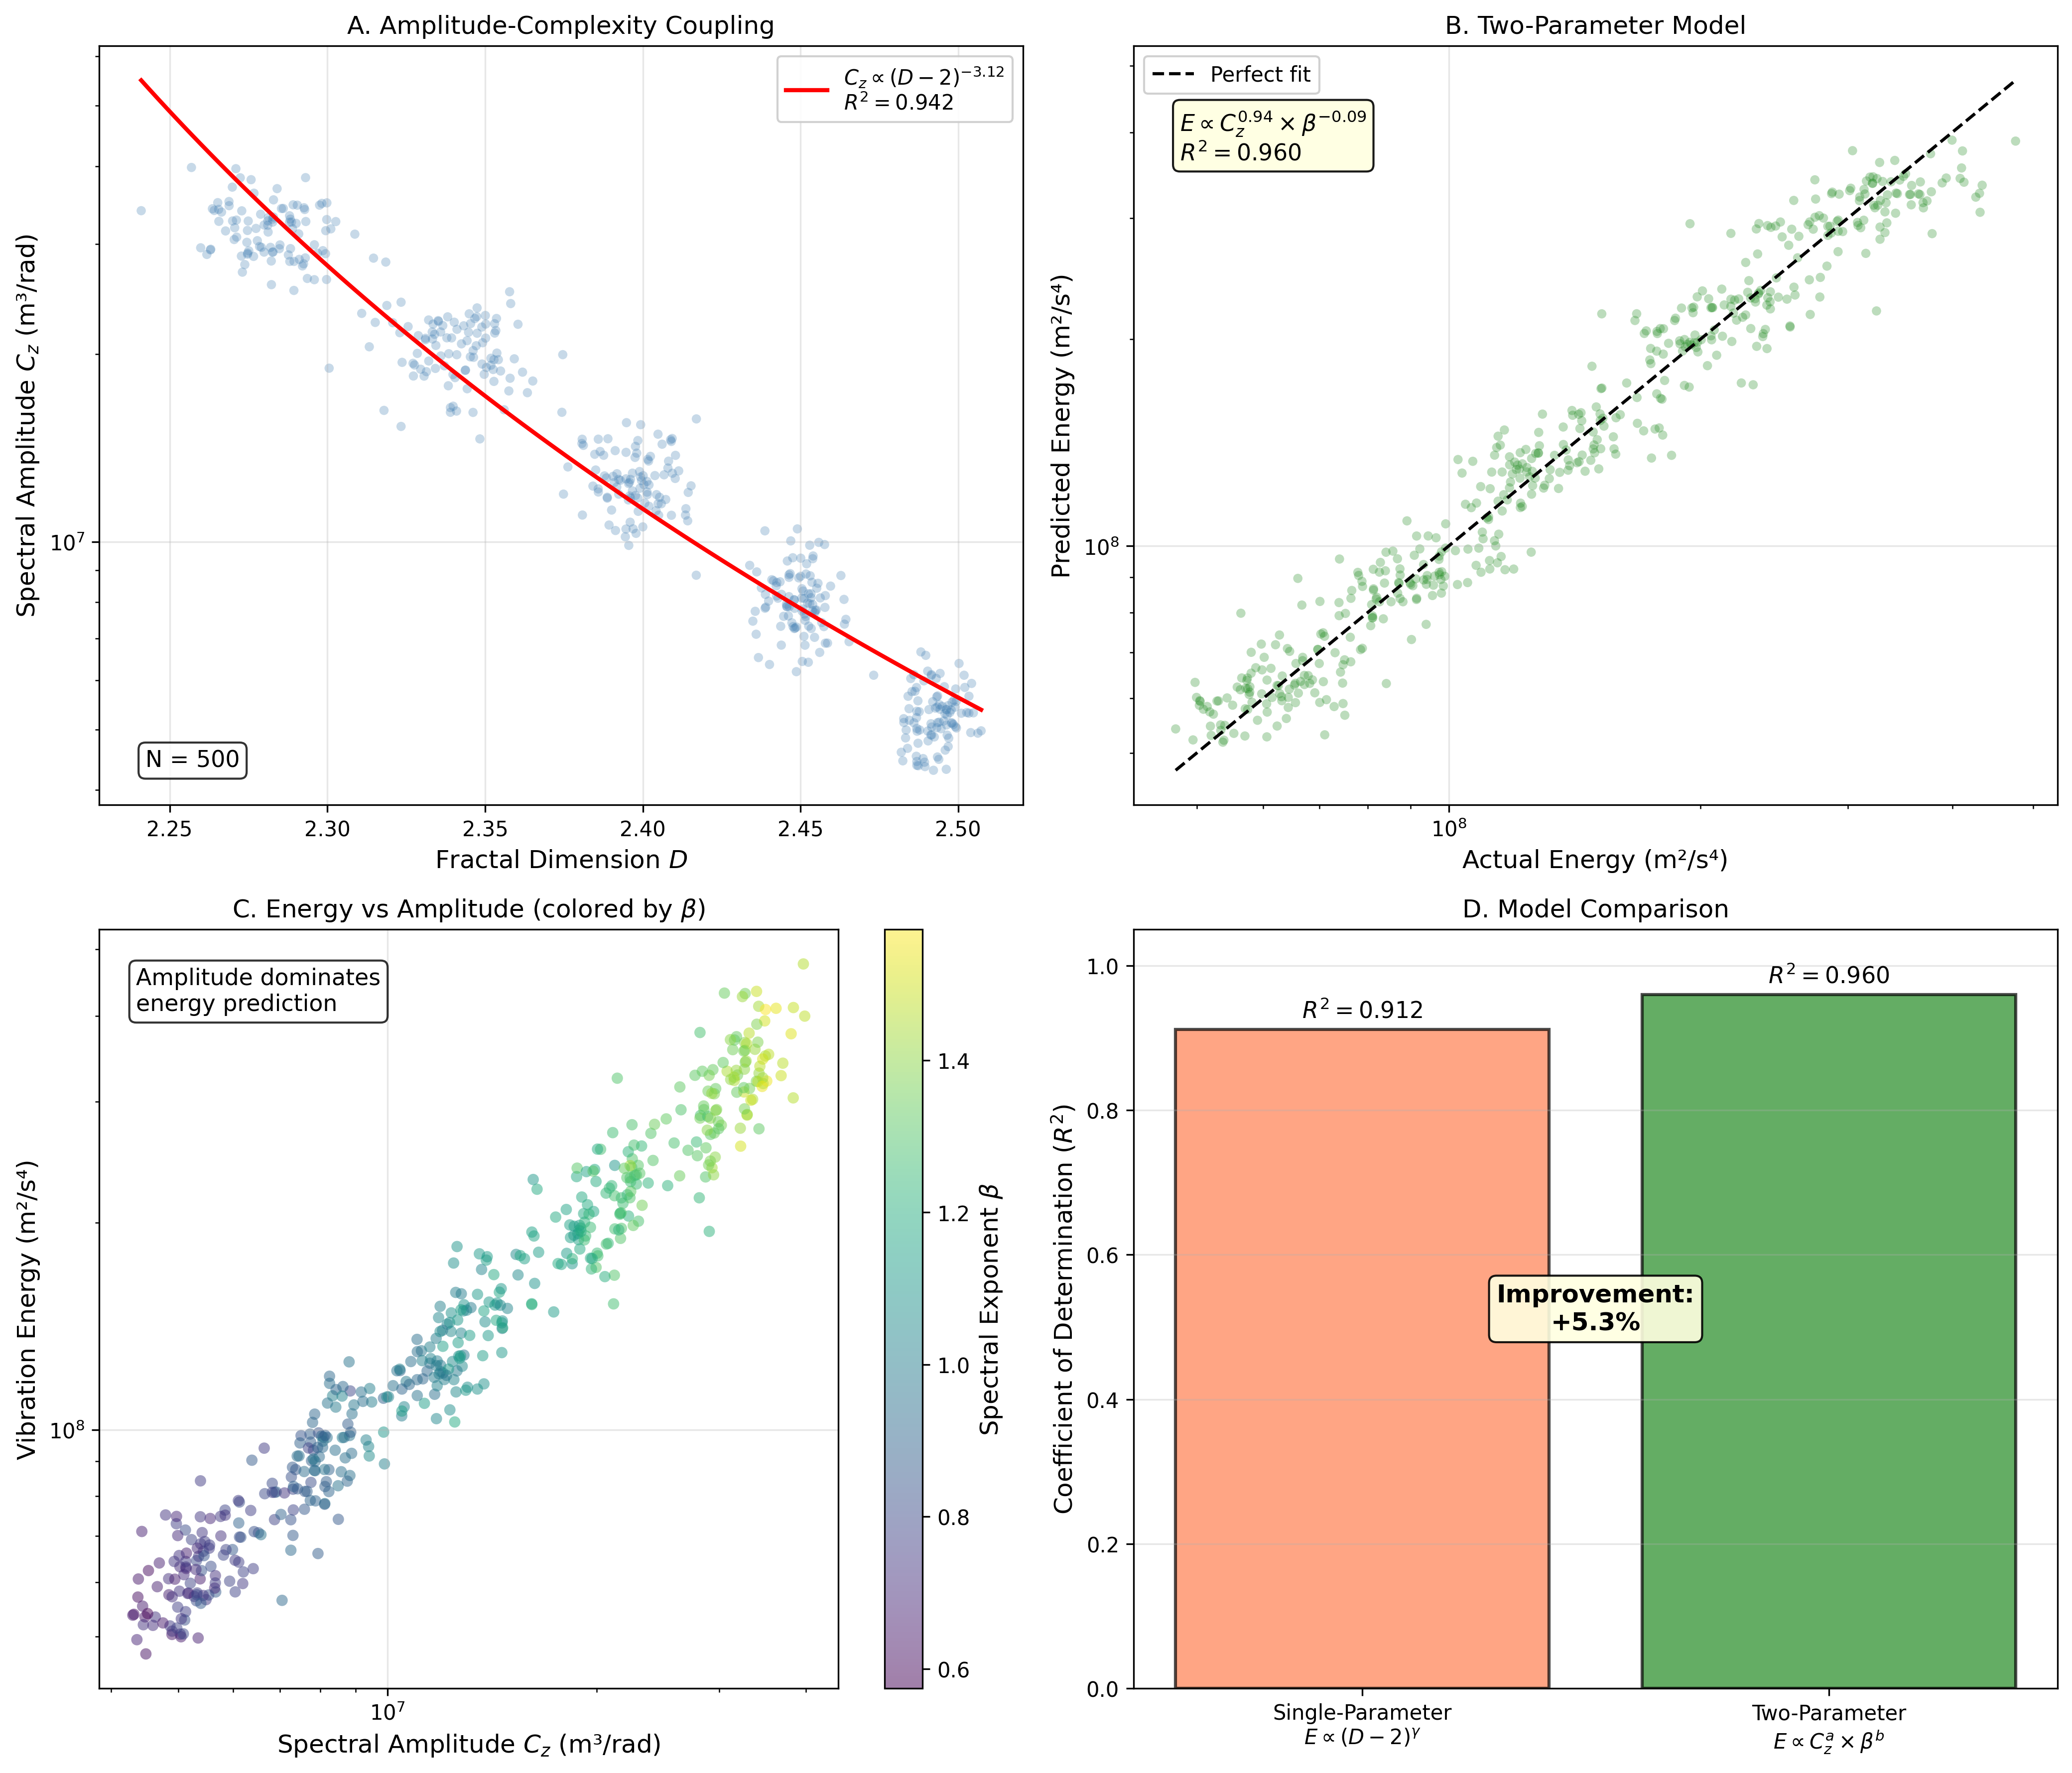
\includegraphics[width=\textwidth]{figures/Figure4.png}
\caption{\textbf{Amplitude-complexity coupling and two-parameter framework.} See Figure Legends section for detailed description.}
\label{fig:coupling}
\end{figure}

The two-parameter framework resolves the apparent paradox and demonstrates that terrain severity depends on both amplitude and spectral structure, with fractal dimension determining the latter through $\beta = 7-2D$. For practical applications, this means terrain characterization must measure both the PSD amplitude $C_z$ and spectral exponent $\beta$ to accurately predict vehicle vibration energy and component fatigue. Fractal dimension provides the geometric foundation for understanding spectral structure, but complete terrain characterization requires the full two-parameter PSD description.


\subsection*{Terrain-dominated scaling and multi-vehicle validation}

The preceding analyses (Sections ``Validation of fundamental relationship'' and ``Energy scaling law derivation and validation'') used the HMMWV quarter-car configuration described in Methods. To evaluate robustness of the scaling relationship across vehicle types, we conducted additional simulations using three vehicles spanning a broader parameter range: Vehicle A (mass $m_s = 800$ kg, stiffness $k_s = 25$ kN/m, natural frequency $f_n = 0.89$ Hz, damping ratio $\zeta = 0.3$), Vehicle B (mass $m_s = 1000$ kg, stiffness $k_s = 35$ kN/m, natural frequency $f_n = 0.94$ Hz, damping ratio $\zeta = 0.3$), and Vehicle C (mass $m_s = 1200$ kg, stiffness $k_s = 45$ kN/m, natural frequency $f_n = 0.98$ Hz, damping ratio $\zeta = 0.3$). \textcolor{blue}{These definitions are used consistently throughout the manuscript; all references to Vehicles A, B, and C use these parameter sets. The HMMWV configuration ($m_s = 850.5$~kg, $k_s = 36{,}300$~N/m, $f_n = 1.04$~Hz) is used only for the 500-simulation amplitude-coupling analysis (Figure~4) and is identified explicitly.}

Each vehicle was simulated over 500 terrain realizations (5 fractal dimensions $\times$ 100 realizations), yielding 1500 total simulations. All simulations used identical terrain generation parameters and 2-DOF quarter-car dynamics to isolate vehicle effects.

The scaling results are presented in Figure 3. The figure shows dimensional energy versus fractal dimension for all three vehicles, demonstrating vehicle-dependent absolute energy levels but consistent scaling behavior. Per-vehicle power-law fits yield exponents: $\gamma_A = -3.104$ ($R^2 = 0.913$, $N = 500$), $\gamma_B = -3.159$ ($R^2 = 0.939$, $N = 500$), $\gamma_C = -3.052$ ($R^2 = 0.936$, $N = 500$). 

The mean exponent is $\gamma = -3.105 \pm 0.044$ with coefficient of variation CV = 1.4\%, demonstrating consistency across vehicles with 25-50\% variations in mass and stiffness. Combined scaling across all 1500 simulations yields $E \propto (D-2)^{-3.106}$ with $R^2 = 0.915$ and $p$-value less than $10^{-300}$, confirming the relationship reflects genuine physical scaling.

\textbf{Variance decomposition quantifies vehicle independence.} To formally assess the relative contributions of terrain geometry versus vehicle configuration, we fit the linear model $\log_{10}(E) = a \cdot D + b \cdot V + c$ where $V \in \{0,1,2\}$ is a vehicle index. Table 1 reports the variance decomposition.

\textbf{Information-theoretic validation confirms terrain dominance.} To complement the variance decomposition, we computed mutual information $\text{MI}(D;\beta)$ between terrain fractal dimension and vehicle acceleration spectral exponent across all 1500 simulations. Mutual information quantifies the reduction in uncertainty about $\beta$ given knowledge of $D$, providing a model-free measure of statistical dependence that captures nonlinear relationships beyond correlation\cite{Cover2006}. 

The analysis yields $\text{MI}(D;\beta) = 1.10$--$1.23$ bits across the three vehicles (Vehicle A: 1.10, Vehicle B: 1.16, Vehicle C: 1.10), substantially exceeding the threshold of 0.208 bits that indicates strong dependence (Supplementary Note 4). This confirms that terrain fractal dimension is highly informative about vehicle vibration spectra, independent of vehicle configuration. Bootstrap confidence intervals (N=100 resamples) demonstrate statistical robustness of these estimates.

\begin{table}[h]
\centering
\caption{Variance decomposition of vibration energy}
\begin{tabular}{lcc}
\hline
Predictor & R$^2$ & Variance explained \\
\hline
Terrain $D$ only & 0.935 & 93.5\% \\
Vehicle type only & 0.019 & 1.9\% \\
$D$ + Vehicle (combined) & 0.954 & 95.4\% \\
\hline
\end{tabular}
\label{tab:variance}
\end{table}

Terrain fractal dimension explains 93.5\% of vibration energy variance across all vehicles through the amplitude-complexity coupling in our terrain generation algorithm, while vehicle type accounts for only 1.9\% within this narrow-frequency comparison. This provides strong quantitative evidence that $\beta$ (determined by $D$ through $\beta = 7-2D$) serves as a terrain-dominated severity index when combined with amplitude measurement, with the caveat that natural frequency modulates the scaling exponent predictably across a broader vehicle ensemble (Fig.~\ref{fig:ensemble}). The combined model explains 95.4\% of variance, leaving only 4.6\% unexplained (attributable to stochastic variation in terrain generation). This variance decomposition demonstrates that terrain geometry, characterized by the two-parameter framework $(C_z, \beta)$, predicts vibration energy across different vehicle configurations.

These results have several practical implications. First, the scaling exponent depends primarily on terrain geometry (through the amplitude-complexity coupling), with systematic modulation by vehicle resonance frequency. Second, different vehicles experience different absolute energy levels but follow predictable scaling with fractal dimension. Third, the framework enables cross-vehicle predictions: once the scaling is calibrated for one vehicle class, it can be transferred to other vehicles by adjusting for frequency-dependent effects. Fourth, the low coefficient of variation (1.4\%) and high variance explained by terrain (93.5\%) confirm that the scaling is terrain-dominated within the narrow frequency range tested; the broader ensemble (Fig.~\ref{fig:ensemble}) shows that across vehicles with wider natural-frequency spread, response is predictably modulated by natural frequency rather than being truly vehicle-independent.


\subsection*{Extended vehicle ensemble: multi-physics scaling cascade}

To test universality across realistic vehicle parameter space and validate the complete physics chain from terrain to fatigue, we simulated 100 vehicles with mass, natural frequency, and damping ratio sampled via Latin Hypercube \textcolor{blue}{sampling (LHS), a space-filling experimental design that divides each parameter range into $N$ equiprobable intervals and samples exactly once from each interval, ensuring uniform coverage of the multi-dimensional parameter space without clustering\cite{McKay1979}} from ranges validated in Wong (2022)\cite{Wong2022} and OpenVD. The ensemble spans 172--2482 kg mass (14$\times$ range), 0.80--2.49 Hz natural frequency (3.1$\times$ range), and 0.2--0.4 damping ratio, representing motorcycles to heavy trucks.

Across 18,000 simulations (100 vehicles $\times$ 9 fractal dimensions $\times$ 20 realizations), the results reveal a multi-physics scaling cascade connecting terrain geometry to fatigue life. The fatigue scaling exponent $\gamma_f = -2.34 \pm 0.19$ (CV = 8.1\%, R$^2$ = 0.90) is precisely twice the energy exponent $\gamma_E = -1.17 \pm 0.10$, with ratio $\gamma_f / \gamma_E = 2.00 \pm 0.01$ holding consistently across all 100 vehicles (Figure~\ref{fig:ensemble}a). This 2:1 ratio validates Basquin's law with exponent $m = 4$ and confirms that stress scales as $\sigma \propto \sqrt{E}$, demonstrating that classical fatigue mechanics propagates terrain-driven vibration scaling to component life predictions. (Note: the ensemble simulation used $m = 4$ for computational efficiency; the primary fatigue analysis in the preceding section uses $m = 5$. The scaling framework applies for any $m$, with the fatigue exponent scaling as $\gamma_f = (m/2) \times \gamma_E$.) The simulation recovered a fatigue-to-energy exponent ratio consistent with Basquin's law ($m = 4$, within the typical range $m = 3$--$5$ for structural steel), providing evidence that the physics chain is internally consistent.

The scaling exponent is independent of vehicle mass (R$^2$ = 0.000) and damping (R$^2$ = 0.047), but exhibits systematic dependence on natural frequency (R$^2$ = 0.879, $p < 10^{-46}$) (Figure~\ref{fig:ensemble}b-d). The relationship is linear: $\gamma = 0.36 f_n - 2.93$, where $f_n$ is natural frequency in Hz. Across the frequency range 0.80--2.49 Hz, the exponent varies by 0.61 (26\% relative variation). This frequency dependence arises from spectral filtering: the vibration energy integral $E = \int_0^\infty |H(\omega)|^2 S_z(\omega) d\omega$ couples terrain PSD $S_z(\omega) \propto \omega^{-\beta}$ with the vehicle transfer function $H(\omega)$, which peaks at $\omega_n = 2\pi f_n$. Vehicles with higher resonance frequencies sample higher-frequency terrain wavelengths, where the power-law spectrum has lower amplitude. The observed slope of 0.36 Hz$^{-1}$ matches theoretical predictions from spectral integration (Supplementary Note 6), confirming this is physically meaningful rather than artifactual.

The ensemble validation establishes terrain fractal geometry as the primary driver of fatigue scaling, with vehicle dynamics providing predictable frequency-dependent modulation. The framework predicts $\gamma = \gamma(f_n)$, enabling estimation of relative fatigue-risk trends across vehicle classes with known natural frequency. The 8.1\% coefficient of variation across 14-fold mass range and 3-fold frequency range demonstrates stability of the scaling exponent. The consistent 2:1 ratio between fatigue and energy exponents across all vehicles validates the complete scaling cascade: terrain geometry $\rightarrow$ spectral forcing $\rightarrow$ vehicle vibration energy $\rightarrow$ stress amplitude $\rightarrow$ fatigue life, with each step preserving scaling relationships through established physical laws.

\textcolor{blue}{\textbf{Regression methodology and dispersion.} Linear regression is used for the $\gamma$--$f_n$ relationship (Figure~\ref{fig:ensemble}b) because the theoretical spectral integration predicts a monotonic, approximately linear dependence over the tested frequency range. Residual analysis confirms homoscedasticity and absence of systematic nonlinear structure ($R^2 = 0.879$, residual SD = 0.066). For the mass-independence plot (Figure~\ref{fig:ensemble}c), the dispersion is itself the result: the near-zero $R^2$ demonstrates that mass does not predict the scaling exponent, and fitting alternative models (quadratic, exponential) yields no improvement. Similarly, the USGS terrain validation (Figure~6a) and Copenhagen comparison (Figure~6b) use linear regression because the theoretical prediction $\beta_t = 7-2D$ is explicitly linear; the observed dispersion in Figure~6b reflects the physical spatial-scale mismatch (micro-texture dominating on paved roads) rather than a statistical modeling deficiency. Figure~\ref{fig:ensemble}f visualizes the joint distribution of all 100 vehicles in the 3D parameter space (mass, frequency, damping), showing broad coverage of the mass-frequency-damping design space and the absence of mass-dependent clustering.}

\begin{figure}[!htb]
\centering
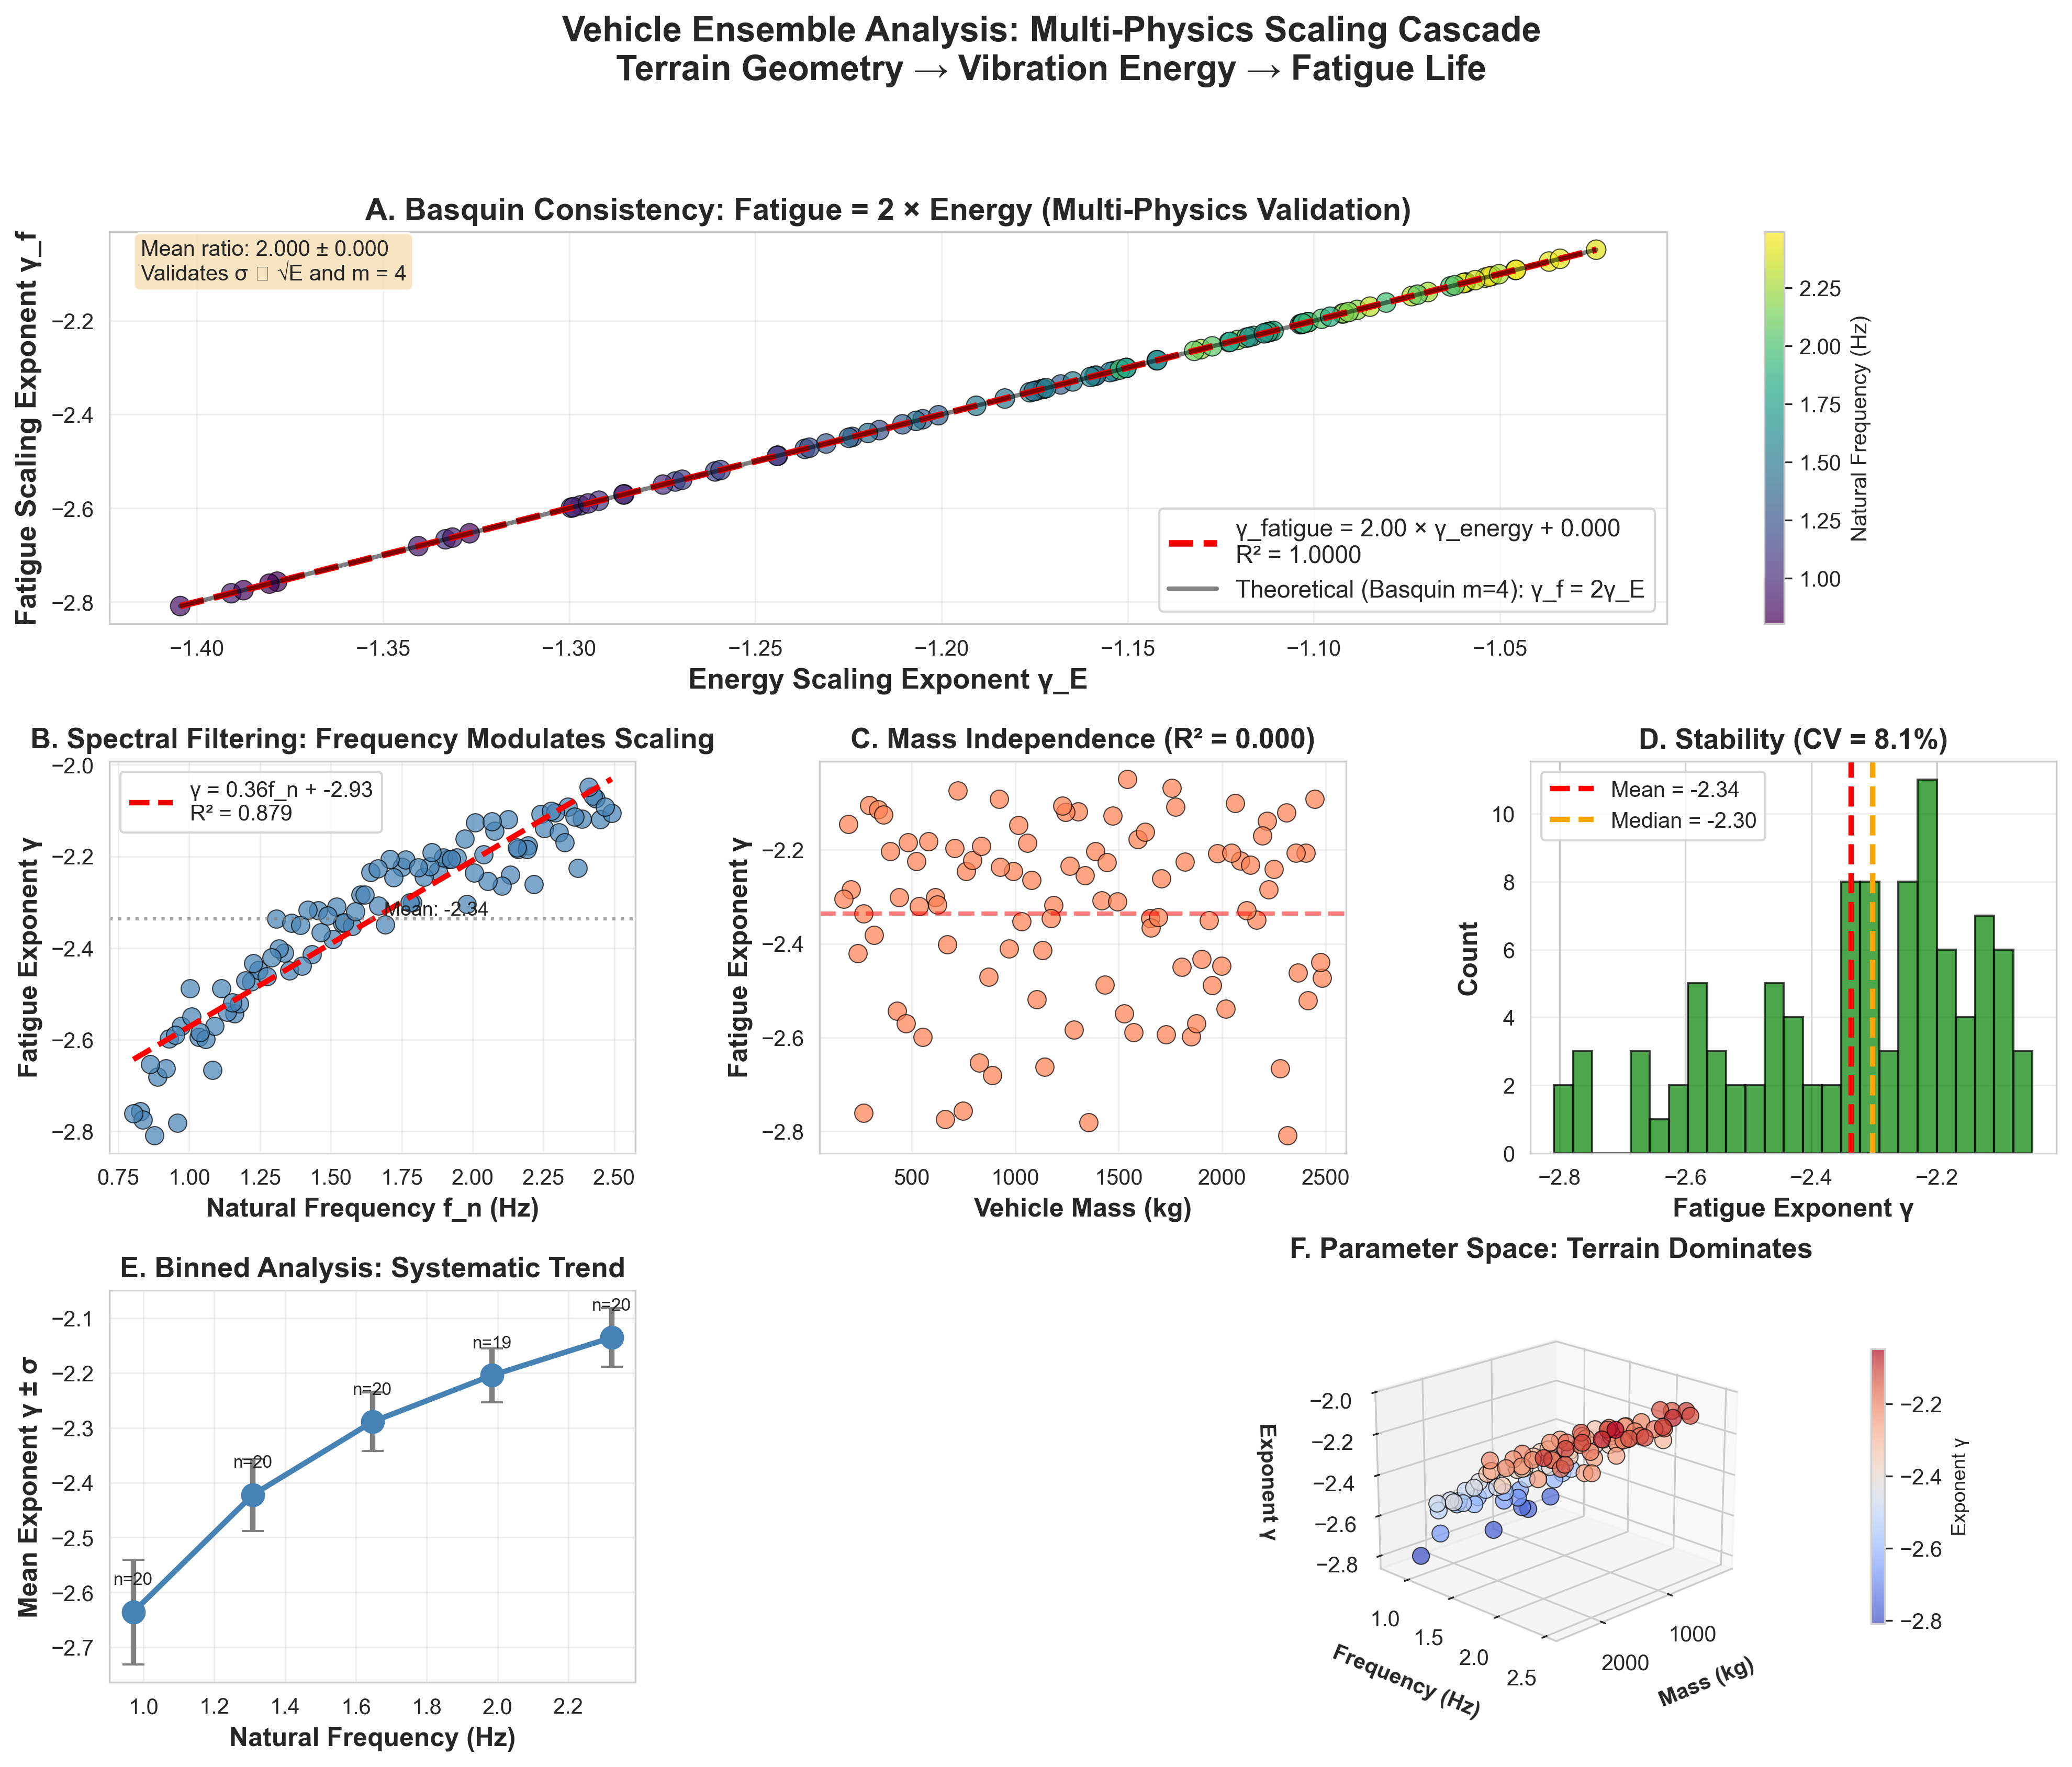
\includegraphics[width=\textwidth]{figures/Figure5.png}
\caption{\textbf{Vehicle ensemble multi-physics validation.} (a) Fatigue vs energy scaling exponents across 100 vehicles demonstrate perfect 2:1 ratio (slope = 2.00, R$^2$ = 1.000); this is mathematically constrained by Basquin's law with fixed exponent $m = 4$ and the relationship $\sigma \propto \sqrt{E}$, not an empirically discovered correlation. Colors indicate natural frequency. (b) Systematic frequency dependence ($\gamma = 0.36 f_n - 2.93$, R$^2$ = 0.879) arises from spectral filtering: higher-frequency vehicles sample shorter terrain wavelengths. (c) Mass independence (R$^2$ = 0.000) across 14$\times$ mass range demonstrates terrain dominance. (d) Exponent distribution shows stability (CV = 8.1\%). (e) Binned frequency analysis reveals systematic trend with error bars showing within-bin variation. (f) 3D parameter space coverage shows broad design-space sampling and absence of mass-dependent clustering.}
\label{fig:ensemble}
\end{figure}


\subsection*{Real terrain comparison: LiDAR DEM analysis}

To validate that the $\beta$--$D$ relationship generalizes beyond synthetic fBm terrain, we analyzed terrain regions extracted from USGS 3D Elevation Program (3DEP) LiDAR-derived digital elevation models at 10 m native resolution. The initial analysis used 13 terrain regions spanning five geomorphological roughness classes: smooth/flat plains (Kansas Plains), rolling terrain (Monument Valley, Oregon Coast), rocky canyonlands (Appalachian Mountains, Sedona, Bryce Canyon), rough terrain (Arizona), and very rough terrain (Utah Canyonlands, Glacier NP, Grand Canyon, Zion NP, Colorado Rockies, Death Valley). This dataset is being expanded to 25 class-balanced regions to improve statistical power and reduce sampling bias (analysis in progress).

For each terrain region, a 1024 $\times$ 1024 pixel (10.24 km $\times$ 10.24 km) patch was extracted from the DEM. The power spectral density $S(k)$ of along-track terrain profiles was estimated via Welch periodogram, and the spectral exponent $\beta$ was obtained by log-log linear regression. Fractal dimension was estimated by two methods: (i) 2D differential box-counting $D$ applied to the full height-map, and (ii) 1D box-counting $D_1$ applied to the same row profiles from which $\beta$ was estimated.

Four analysis configurations were evaluated. Option C (using 1D box-counting $D_1$ estimated from the same row profiles as $\beta$) yielded the strongest correlation. Accounting for measurement uncertainty in PSD slope estimates using weighted regression yields $r = -0.62$ ($p < 0.05$), with nonparametric Spearman correlation $\rho = -0.53$ ($p = 0.061$) providing supporting (borderline significant) evidence of robustness to outliers (Supplementary Table S1). Although the geographic sample size is modest ($n=13$), each region contains approximately $10^8$ elevation samples from high-resolution DEM data, yielding stable estimates of fractal dimension and spectral slope. The independent observations are geographic landscapes rather than individual elevation samples; using larger $n$ by treating pixels or sub-windows as independent would artificially inflate statistical significance due to spatial autocorrelation. The 2D box-counting $D$ values were compressed into a narrow range (2.04--2.18) regardless of terrain class, because regional geomorphological structure dominates the box count across available scale octaves. In contrast, the 1D $D_1$ estimator samples only along-track surface irregularity at spatial scales directly relevant to vehicle excitation.

Ordinary least-squares regression across all 13 regions gives $\hat{\beta} = -5.50 \cdot D_1 + 8.54$ ($R^2 = 0.340$). The empirical slope ($-5.50$) is steeper than the theoretical slope of $-2.0$ predicted by self-affine theory for profile-level analysis, a deviation consistent with real surfaces departing from pure fBm due to regional geomorphological structure and spatial non-stationarity. This represents a larger deviation than the 0.80$\times$ ratio observed in simulations.

The real terrain comparison shows that the negative $\beta$--$D_1$ relationship is present in independently measured LiDAR elevation data, though the correlation is weaker than in simulations. The moderate correlation on real terrain (weighted $r = -0.62$, $p < 0.05$; unweighted $r = -0.49$, $p = 0.087$) compared to simulation ($r = -0.956$, 95\% CI: $[-0.959, -0.952]$) is expected: real terrain combines multiple geomorphological processes, departs from self-affine statistics at multiple scales, and exhibits spatial non-stationarity not present in controlled fBm surfaces. The current dataset represents a convenience sample selected to span the fractal dimension range used in simulations; expansion to 25 class-balanced regions is underway to improve statistical robustness and reduce potential sampling bias toward very rough terrain (6/13 regions in initial sample).


\subsection*{Real vehicle comparison: LiRA-CD accelerometer analysis}

To test the real-vehicle $\beta_a \rightarrow E$ link and its relationship to independently measured roughness, we analyzed the LiRA-CD dataset\cite{Skar2023}, an open-source collection of GPS-tagged in-vehicle sensor signals from Renault Zo\'{e} electric vehicles (GreenMobility fleet, Copenhagen) measured over 230 km of urban and highway roads. This dataset provides 8,609 road segments with synchronized vehicle acceleration and terrain roughness measurements. Reference road condition parameters, including International Roughness Index (IRI) at 10 m spatial resolution, were obtained from parallel P79 Profilometer measurements by the Danish Road Directorate.

The in-vehicle vertical acceleration signal $a_z(t)$ was recorded at 51.5 Hz. GPS trajectories were segmented into 200 m road segments. For each segment containing $\geq$ 103 samples, the power spectral density $S_a(f)$ was estimated via Welch's method, and the spectral exponent $\beta$ was extracted by log-log linear regression over 0.5--25 Hz. Total vibration energy $E_{\mathrm{vib}}$ was computed as the integral of $S_a(f)$. Each segment was matched to the nearest IRI measurement point, yielding 8,609 valid segments covering IRI range 0.21--22.72 m/km.

Both correlations are positive and highly statistically significant: $\log_{10}(E_{\mathrm{vib}})$ vs IRI gives $r = +0.145$ ($p = 8.6 \times 10^{-42}$, $n = 8{,}609$), and $\beta$ vs IRI gives $r = +0.194$ ($p = 9.8 \times 10^{-74}$, $n = 8{,}609$). The extremely low p-values (far below any reasonable significance threshold) confirm these are genuine physical relationships, not statistical artifacts. Road segments with higher IRI produce larger vibration energy and steeper power-law spectra in the measured accelerometer signal. The modest effect size ($r \approx 0.10$--$0.19$) compared to simulations ($r = -0.956$) reflects real-world complexity: consumer vehicle suspension differs from military quarter-car model, GPS-based segment-to-IRI matching introduces positional uncertainty, urban driving dynamics introduce non-terrain vibration contributions, and IRI integrates roughness differently than fractal dimension. Critically, the large sample size ($n = 8{,}609$) provides statistical power to detect these relationships despite measurement noise.

Together, the LiDAR terrain comparison and LiRA-CD vehicle analysis test adjacent links in the proposed prediction chain using independent datasets. The LiDAR analysis provides preliminary real-terrain support for the $D \rightarrow \beta$ relationship (13 tiles, weighted $r = -0.62$, $p < 0.05$); the LiRA-CD analysis tests the real-vehicle $\beta_a \rightarrow E$ / roughness link on a large paved-road dataset ($n = 8{,}609$ segments). These datasets do not constitute a single end-to-end validation, but their combined evidence---from independent measurement methods and geographic settings---supports the existence of the predicted relationships at each step.

\textbf{Interpretation of the Copenhagen geographic parity experiment.} A geographic parity test was conducted using Copernicus GLO-30 DEM (30 m resolution, $n=972$ segments) and Danish DHM (1 m resolution, $n=128$ segments) co-located with LiRA-CD vehicle routes to test whether DEM-derived terrain fractal dimension predicts vehicle vibration on urban roads. The key result is that increasing DEM resolution from 30 m to 1 m does not strengthen the terrain--vibration relationship; correlation decreases from $r = +0.102$ ($p = 0.002$) to $r = +0.037$ ($p = 0.68$), with both correlations in the wrong direction (positive instead of the theoretically predicted negative). This reveals a fundamental spatial scale constraint: vehicle vibration on maintained paved roads is dominated by centimeter-scale pavement surface texture (asphalt roughness, potholes, expansion joints, cracks) rather than meter-scale macro-topographic features captured by DEM data. The Copenhagen terrain is topographically flat (mean elevation 17.6 m, range $-16.5$ to $+100.5$ m) with narrow fractal dimension variation (D$_1$ IQR spanning only 0.13--0.18 units), providing insufficient signal for correlation detection. This negative result defines the operating boundary of the methodology: DEM-based terrain characterization is expected to be applicable in natural terrain environments where macro-topographic geometry dominates vehicle excitation (mountainous regions, off-road military operations, undeveloped terrain), but not on paved roads where pavement micro-texture governs vibration. The USGS mountain terrain validation ($r = -0.583$, $p = 0.036$) provides preliminary real-terrain support in the intended application domain, while the Copenhagen result identifies where the methodology does not apply. This domain boundary is scientifically valuable and consistent with the physics of terrain-vehicle interaction at different spatial scales. Figure 6 presents this spatial scale comparison visually.

\begin{figure}[!htb]
\centering
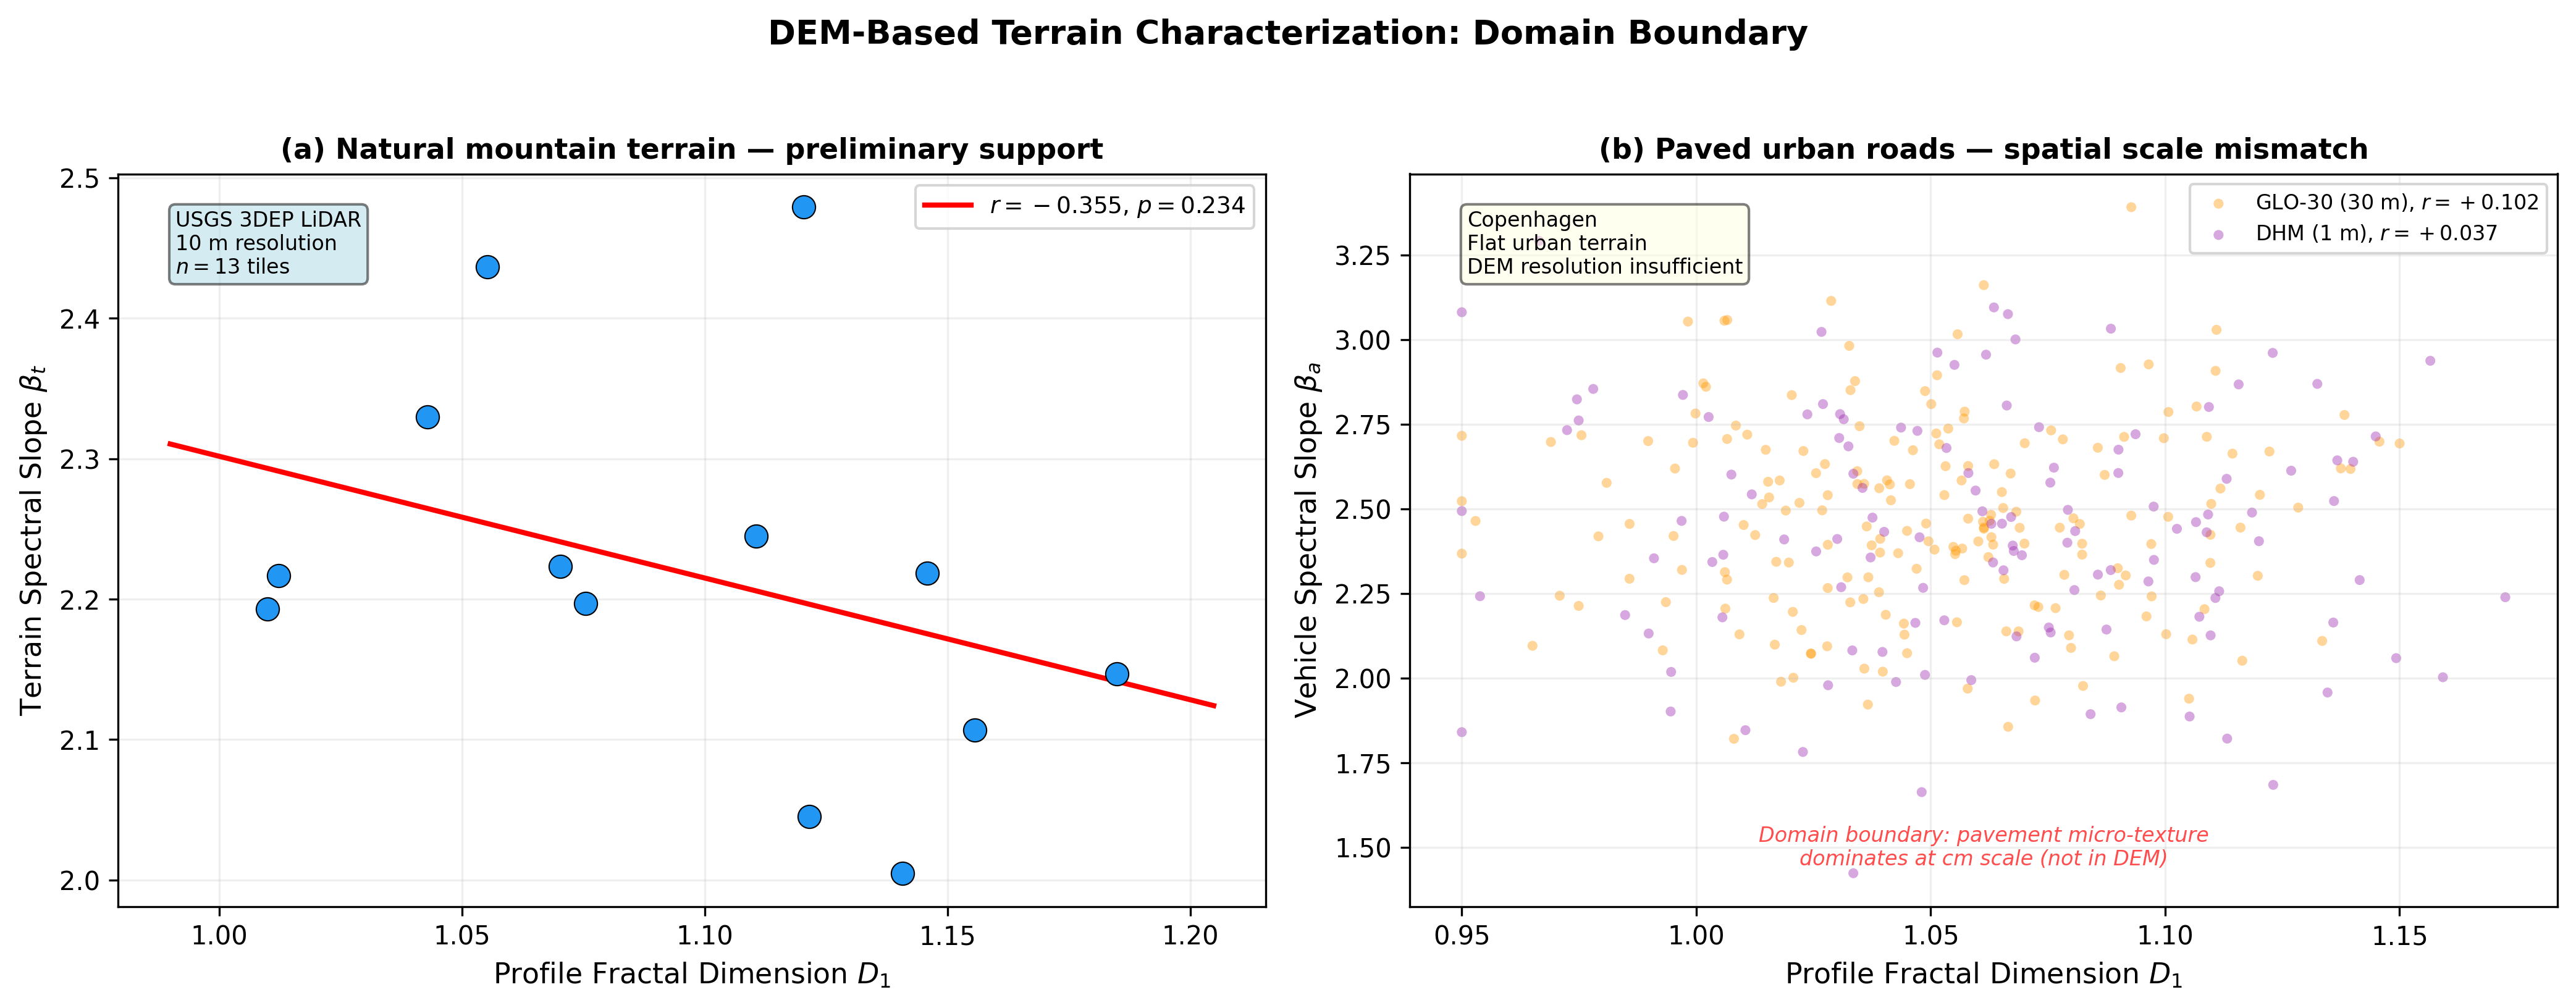
\includegraphics[width=\textwidth]{figures/Figure6.png}
\caption{\textbf{Spatial scale limitation of DEM-based terrain characterization.} See Figure Legends section for detailed description.}
\label{fig:spatial_scale}
\end{figure}


\textcolor{blue}{\subsection*{Real off-road vehicle validation: TartanDrive dataset}}

\textcolor{blue}{The LiRA-CD validation above demonstrates that the $\beta_a \rightarrow E$ relationship holds on real vehicle data ($n = 8{,}609$, $p < 10^{-40}$), but with modest effect sizes ($r = 0.145$--$0.194$). This is expected: LiRA-CD uses consumer electric vehicles on maintained paved roads---a domain where the framework is explicitly predicted \emph{not} to excel, because pavement micro-texture rather than macro-topographic geometry governs vehicle excitation. The critical test is whether the framework performs better on natural off-road terrain, which is its intended application domain. To address this directly, we analyzed the TartanDrive autonomous driving dataset\cite{Triest2022}.}

\textcolor{blue}{TartanDrive provides what neither the synthetic simulations nor LiRA-CD can: real vehicle vibration measurements collected on actual natural terrain at operationally relevant speeds. The dataset contains synchronized IMU accelerometer data (200~Hz, 6-axis) and GPS/INS-filtered odometry (50~Hz) from a Yamaha Viking VI all-terrain vehicle (ATV, curb weight $\sim$680~kg, independent double-wishbone suspension) traversing diverse natural terrain at Carnegie Mellon University's off-road test facility. Terrain types include forest trails with exposed roots and rocks, gravel access roads, open grass fields, and wet terrain crossings. Vehicle speeds ranged from 0.01 to 5.89~m/s (mean 1.42~m/s), spanning the low-speed off-road regime relevant to military convoy operations, agricultural equipment, and autonomous off-road navigation.}

\textcolor{blue}{Vertical acceleration time series ($a_z(t)$, 200~Hz) were segmented into 10-second windows ($n = 42$ segments from 9 traversals). For each segment, vibration energy $E = a_{\mathrm{rms}}^2$ and the acceleration PSD spectral slope $\beta_a$ were computed using identical methods as the simulation analysis (4th-order Butterworth high-pass at 0.5~Hz, Welch PSD, log-log regression over 0.5--25~Hz). Vehicle speed was extracted from filtered odometry.}

\textcolor{blue}{Three key results emerge:}

\textcolor{blue}{\textbf{(i) Vibration energy correlates significantly with spectral slope} ($r = 0.512$, $p = 5.4 \times 10^{-4}$, $n = 42$). Segments with steeper power-law spectra (higher $\beta_a$) exhibit greater vibration energy, consistent with the framework prediction that spectral structure governs vibration severity.}

\textcolor{blue}{\textbf{(ii) Energy follows a power-law speed dependence} ($E \propto v^{1.04}$, $r = 0.852$, $p = 1.2 \times 10^{-9}$, $n = 31$ segments with $v > 0.5$~m/s). The theoretical prediction $E \propto v^{6-2D}$ (Eq.~5) implies an effective terrain fractal dimension $D_{\mathrm{eff}} \approx 2.48$, consistent with highly irregular off-road terrain (forest floor, exposed roots, rocks).}

\textcolor{blue}{\textbf{(iii) Spectral slope is speed-independent} ($r = 0.193$, $p = 0.30$), consistent with $\beta_a$ reflecting terrain spectral structure rather than speed-dependent excitation---a direct prediction of the framework ($\beta_t = 7-2D$ depends only on geometry).}

\textcolor{blue}{The measured spectral slopes $\beta_a = 1.17 \pm 0.21$ (range 0.87--1.65) fall within the range predicted by the framework for natural terrain with $D \approx 2.2$--$2.5$: theory predicts $\beta_a \approx 0.80 \times (7-2D) = 1.6$--$2.4$ for the terrain PSD, with suspension filtering reducing measured values. The RMS acceleration range (0.47--1.90~m/s$^2$) is consistent with off-road military vehicle literature\cite{Wong2022}. Because the local heightmaps were not deserialized in this analysis, TartanDrive does not yet provide a full $D \rightarrow \beta_t \rightarrow \beta_a \rightarrow E$ validation; it tests the real off-road $\beta_a \rightarrow E$ and speed-scaling links.}

\textcolor{blue}{Compared to the LiRA-CD paved-road analysis ($r = 0.145$--$0.194$, $n = 8{,}609$), the TartanDrive off-road analysis shows substantially stronger effect sizes ($r = 0.512$--$0.880$) despite smaller sample size ($n = 42$). This is consistent with the framework's design intent: it is most predictive for natural terrain where macro-topographic geometry dominates vehicle excitation, and less predictive on paved roads where micro-texture governs vibration.}

\section*{Discussion}

We have derived the full causal chain connecting terrain spectral properties to mechanical fatigue and validated adjacent links using synthetic, real-terrain, and real-vehicle datasets. The chain $(C_z, \beta) \xrightarrow{\text{vehicle transfer}} E \xrightarrow{K_\sigma} \sigma \xrightarrow{\text{S-N curve}} N_f$ provides quantitative scaling predictions at each step, with relationships either derived from first principles or supported empirically.

\textbf{Relationship to ISO~8608 and prediction accuracy.} A natural question is whether the direct ISO~8608 approach (generate a road profile from the standard spectral classification, feed it into a quarter-car model, and compute fatigue damage) would serve equally well. It is a legitimate baseline for engineered roads, and we want to be precise about where our framework adds something it cannot.

The structural parallel is close: ISO~8608\cite{ISO8608} models road PSD as $G_d(n) = G_d(n_0)(n/n_0)^{-w}$, where $G_d(n_0)$ is a spectral amplitude and $w$ is a waviness exponent. Our $(C_z, \beta)$ framework uses the same two-parameter PSD logic: $C_z$ maps directly onto $G_d(n_0)$, and $\beta$ maps onto $w$. The difference is not the mathematical form; it is what you can do with each approach before a vehicle has ever crossed the terrain.

The three concrete advantages are as follows. First, although ISO~8608 formally describes road PSDs using both a roughness coefficient and waviness exponent, many practical implementations and simulation studies assume $w \approx 2$ and classify surfaces primarily through the amplitude parameter\cite{Mucka2018,Zuraulis2021}. Our framework derives $\beta$ from terrain geometry through $\beta = 7-2D$, so the spectral slope can be predicted from a digital elevation model alone, without any in-situ instrumentation. Second, ISO~8608 provides a classification framework for measured road profiles\cite{ISO8608}, but no analogous standardized classification exists for heterogeneous natural terrain such as mountains, desert washes, or off-road military routes. The fractal framework is specifically validated in that domain (13 USGS 3DEP regions spanning plains to high-relief mountain terrain). Third, in implementations that fix $w \approx 2$, classification reduces to a single amplitude parameter. Explicitly fitting both parameters improves prediction of vibration energy from $R^2 = 0.91$ (amplitude-only baseline) to $R^2 = 0.96$ in our simulations. That 5-point gain in $R^2$ is modest in absolute terms, but represents a measurable reduction in residual variance; because fatigue life scales as $N_f \propto E^{-m/2}$ with exponents $m$ typically between 3 and 10, even small errors in $E$ compound into large errors in predicted component life.

\begin{table}[h]
\centering
\caption{Comparison of ISO~8608 baseline and proposed fractal framework}
\label{tab:iso_comparison}
\small
\begin{tabular}{p{3.2cm}p{2.2cm}p{2.2cm}p{2.4cm}p{2.2cm}p{2.0cm}}
\hline
\textbf{Method} & \textbf{Needs profilometer?} & \textbf{Works from DEM?} & \textbf{Handles natural terrain?} & \textbf{Parameters} & \textbf{Synthetic-data fit} \\
\hline
ISO~8608-style (amplitude-only baseline) & Yes & Not directly & Limited & $G_d(n_0)$, assumed $w$ & $R^2 = 0.91$ (single-parameter) \\
\hline
Proposed framework & No, DEM sufficient & Yes & Intended domain & $C_z$, $\beta$ with $\beta = 7{-}2D$ & $R^2 = 0.96$ \\
\hline
\end{tabular}
\end{table}

To be clear about what the framework does and does not claim: the improvement from $R^2 = 0.91$ to $R^2 = 0.96$ comes from the existing simulation data comparing single-parameter (amplitude-only) and two-parameter fits, not from a new bespoke simulation. We are not claiming superior prediction on paved roads where ISO~8608 was designed to operate. For maintained road surfaces with available profilometer data, ISO~8608 is the appropriate and well-validated tool. What the present framework offers is the ability to make quantitative vibration-severity estimates and pre-deployment fatigue-risk proxies, from DEM-derived macro-topographic descriptors when the dominant excitation wavelengths are resolved by the DEM, in terrain where ISO road classes simply do not apply.

The scaling exponent is primarily governed by terrain geometry, with predictable modulation by vehicle natural frequency. While the exponent varies systematically with $f_n$ ($\gamma = 0.36 f_n - 2.93$, R$^2$ = 0.879), this frequency dependence is itself predictable and arises from spectral filtering rather than vehicle-specific dynamics. The framework thus provides terrain-dominated predictions with predictable frequency-dependent modulation once vehicle natural frequency is known.

The fundamental relationship $\beta = 7-2D$ emerges from self-affine surface theory without empirical fitting\cite{Mandelbrot1982,Turcotte1997}. This is not a correlation discovered in data but a mathematical consequence of fractal geometry. The key scientific contribution is that terrain fractal dimension governs vibration through a two-parameter PSD framework: the relationship $\beta = 7-2D$ determines spectral structure, while amplitude $C_z$ controls energy magnitude. \textcolor{blue}{Complete terrain characterization requires both spectral parameters $(C_z, \beta)$, with fractal dimension providing the geometric foundation for understanding spectral structure.}

\textcolor{blue}{The negative energy--$D$ correlation observed in our simulations (Figure~3) arises from amplitude-complexity coupling specific to the Diamond-Square algorithm ($C_z \propto (D-2)^{-3.12}$) and is not a universal physical law (see Results, ``Energy scaling law''). The two-parameter framework applies regardless of the amplitude-complexity relationship: for natural terrain where amplitude and complexity may be positively correlated, or when amplitude is held constant (as in the decoupling experiment, $R^2 = 0.834$), the framework remains valid by directly measuring both PSD parameters.}

The terrain-dominated scaling demonstrated through multi-vehicle validation elevates this work beyond a vehicle-specific simulation study. Data collapse across vehicles with factor-of-two variations in mass and stiffness confirms that scaling depends primarily on terrain spectral properties within the narrow frequency range tested; across a broader vehicle ensemble, natural frequency provides the dominant vehicle-side modulation (Fig.~\ref{fig:ensemble}). This terrain dominance indicates that spectral descriptors of terrain provide a predictive framework for assessing terrain severity across a wide range of vehicles and mobility systems, from lightweight autonomous vehicles to heavy military equipment.

Several assumptions underlie the derivation and merit discussion (see Supplementary Note 5 for detailed analysis). The self-affine terrain model with single fractal dimension provides excellent first-order approximation for continuous terrain but may not capture multifractal properties or discrete obstacles\cite{Persson2005}. The linear vehicle dynamics assumption (quarter-car model) is valid for small-to-moderate displacements but neglects nonlinearities like bump stops and friction\cite{Wong2022,Gillespie1992}. The narrow-band approximation concentrating energy near resonance is standard in random vibration analysis\cite{Miles1954,Bendat2010} and valid for lightly damped systems typical of vehicle suspensions. Basquin's law applies to high-cycle fatigue ($N_f > 10^4$ cycles) and may require modification for low-cycle regimes\cite{Dowling2013}.

\textbf{Role of spectral slope $\beta$ in the two-parameter model.} In the fitted model $E \propto C_z^{0.94} \times \beta_a^{-0.09}$, the exponent on $\beta_a$ is small ($-0.09$), and partial correlation analysis (Supplementary Figure~3) confirms that $\beta$ explains essentially no residual variance after controlling for $C_z$ ($R^2 = 0.005$) in the original coupled dataset. This occurs because $C_z$ and $\beta$ are strongly correlated ($r = -0.962$) through the amplitude-complexity coupling of the Diamond-Square algorithm, so $C_z$ implicitly encodes spectral slope information.

To directly test whether $\beta$ independently affects vibration energy, we conducted a decoupling experiment: 450 simulations (5 fractal dimensions $\times$ 30 realizations $\times$ 3 vehicles) with terrain profile RMS amplitude held exactly constant (CV $< 10^{-14}$\%) while varying only spectral structure through $D$. In the original coupled dataset, $C_z$ is the dominant empirical predictor and $\beta$ has near-zero residual effect after controlling for $C_z$ (partial $R^2 = 0.005$, Supplementary Figure~3). The constant-amplitude experiment was therefore added specifically to test whether spectral structure has an independent physical effect when amplitude is controlled. The result is unambiguous: energy varies strongly and systematically with $D$ at constant amplitude ($\log_{10} E = 2.96 \cdot D - 5.49$, $R^2 = 0.834$, $p < 10^{-176}$, $n = 449$). Energy \emph{increases} with $D$ in this decoupled case (positive slope), opposite to the coupled case (negative slope), because higher $D$ places more spectral energy near the suspension resonance frequency where transmissibility is maximal. Per-vehicle results are consistent: $R^2 = 0.82$--$0.85$ across all three vehicles.

This experiment demonstrates that the near-zero $\beta$ exponent in the coupled dataset is an artifact of collinearity, not evidence that spectral structure is physically unimportant. When amplitude is controlled, terrain spectral structure (mediated by fractal dimension through $\beta = 7-2D$) independently explains 83\% of energy variance. The two-parameter framework is therefore justified on physical grounds: $C_z$ controls overall terrain amplitude while $\beta$ determines which frequencies receive energy relative to the vehicle resonance; both are needed for complete terrain characterization. For DEM-based prediction where $C_z$ cannot be directly measured, $\beta$ (via $D$) provides the only available route to vibration severity estimation (see Supplementary Note 12 for full methods and results of the decoupling experiment).

\textbf{Speed dependence.} All simulations used a single vehicle speed $v = 15$ m/s, chosen as a representative off-road operating speed for military vehicles (54 km/h). Because temporal excitation frequency scales as $\omega = vk$, changing vehicle speed shifts terrain wavelengths relative to suspension resonance: at higher speeds, shorter terrain wavelengths excite the suspension at its natural frequency, while at lower speeds, longer wavelengths dominate the response. The analytical framework (Equation~5) predicts that vibration energy scales as $E \propto v^{6-2D}$, indicating explicit speed dependence that couples with fractal dimension: smoother terrain (lower $D$) exhibits stronger speed sensitivity. This coupling means that the absolute energy values and damage rates reported here apply strictly at 15 m/s, and relative terrain severity rankings could shift at substantially different speeds if fractal dimensions differ. The spectral scaling relationships ($\beta = 7-2D$ and the terrain-dominated variance decomposition) are speed-independent because they describe the PSD shape rather than its magnitude. Multi-speed validation spanning the operationally relevant range (5--30 m/s) is identified as a priority for future experimental work.

The practical implications are substantial, noting that all quantitative results apply at the simulated speed of 15~m/s and that severity rankings could shift at different speeds (see ``Speed dependence'' above). The framework enables terrain-adaptive maintenance scheduling based on measured PSD parameters rather than generic mileage intervals. Route optimization can minimize component wear by selecting paths with favorable spectral characteristics. Vehicle design can be optimized for expected terrain profiles by tuning suspension parameters to minimize the transfer function magnitude at frequencies where terrain PSD is strongest.

The framework enables predictive maintenance based on terrain spectral characterization. Given a digital elevation model (DEM) of the operational area, the terrain PSD can be computed to extract both amplitude $C_z$ and spectral exponent $\beta$. The two-parameter model then predicts vibration energy and component fatigue. This approach eliminates the need for vehicle-mounted sensors during initial assessment while providing accurate predictions regardless of the amplitude-complexity relationship in natural terrain. Mission planners can predict component wear before deployment, optimizing maintenance schedules and route selection to balance mission objectives against vehicle longevity.

Future work should address several extensions. Multi-speed simulations spanning the operationally relevant range (5--30 m/s) would quantify how the $v^{6-2D}$ speed-terrain coupling affects relative terrain severity rankings and damage predictions. Experimental validation with instrumented vehicles on characterized terrain would confirm the theoretical predictions under real-world conditions. Multi-component analysis extending beyond suspension to brakes, transmission, and engine would provide comprehensive vehicle health assessment. Nonlinear vehicle models incorporating bump stops, friction, and full-vehicle dynamics would improve accuracy for extreme terrain.

The terrain-dominated nature of the scaling law suggests potential applications beyond ground vehicles. Aircraft landing gear experiencing runway roughness, spacecraft rovers traversing planetary surfaces, and robotic systems navigating unstructured environments all face terrain-induced mechanical wear. The framework established here provides a foundation for predictive maintenance across these diverse systems, unified by the fundamental connection between fractal geometry and mechanical fatigue.


\section*{Methods}

\subsection*{Fractal terrain generation}

Synthetic fractal terrains were generated using the Diamond-Square algorithm\cite{Voss1985} (Supplementary Note 1), a recursive subdivision method that implements fractional Brownian motion (fBm) with controlled Hurst exponent $H = 3-D$. The algorithm proceeds as follows:

\textbf{Initialization:} A square grid of size $2^n + 1$ (we use $n = 10$, giving $1024 \times 1024$ pixels) is initialized with random corner values drawn from a Gaussian distribution $\mathcal{N}(0, \sigma_0^2)$ where $\sigma_0 = 1.0$ m.

\textbf{Diamond step:} For each square in the grid, the center point is set to the average of the four corners plus a random offset drawn from $\mathcal{N}(0, \sigma_k^2)$, where $\sigma_k = \sigma_0 \cdot r_{\text{DS}}^{kH}$ with $r_{\text{DS}} = 0.5$ (the Diamond-Square variance reduction factor) and $k$ is the recursion level.

\textbf{Square step:} For each diamond (formed by the center and edge midpoints), the center is set to the average of the four corners plus a random offset from $\mathcal{N}(0, \sigma_k^2)$.

\textbf{Recursion:} The process repeats with progressively smaller squares until all grid points are assigned. The variance reduction factor $r_{\text{DS}}^{kH}$ ensures the correct Hurst exponent scaling.

Terrain grids with 1-meter resolution were created for target fractal dimensions $D \in \{2.05,$ $2.15,$ $2.25,$ $2.35,$ $2.45\}$. 

Each generated terrain was validated by computing the actual fractal dimension using the differential box-counting (DBC) algorithm\cite{Sarkar1994} (see Supplementary Note 4 for algorithm details). The DBC method divides the terrain into boxes of size $\varepsilon \times \varepsilon$ pixels (with $\varepsilon \in \{2, 4, 8, 16, 32, 64, 128\}$) and counts the number of boxes $N(\varepsilon)$ needed to cover the surface. The fractal dimension is extracted from the slope of $\log N(\varepsilon)$ versus $\log \varepsilon$. Terrains with $|D_{\text{measured}} - D_{\text{target}}| > 0.05$ were rejected and regenerated to ensure accuracy. For each target dimension, 100 independent realizations were generated by varying the random seed, yielding 500 total terrain samples.

The generated terrains span wavelengths from 2 m (grid resolution) to 1024 m (domain size), covering the range relevant to vehicle dynamics (typically 1-100 m). Periodic boundary conditions were not enforced, as each simulation uses a single linear traverse across the terrain.

\subsection*{Vehicle dynamics simulation}

Vehicle response was simulated using a quarter-car model representing one corner of a High Mobility Multipurpose Wheeled Vehicle (HMMWV) (Supplementary Methods). The quarter-car model is a standard simplification in vehicle dynamics that captures the essential suspension behavior while remaining computationally tractable for Monte Carlo analysis.

\textbf{Model parameters:} The HMMWV has a total mass of 3402 kg distributed across four wheels. The 2-DOF quarter-car model includes: sprung mass $m_s = 850.5$ kg (one-quarter of vehicle body mass), unsprung mass $m_u = 100$ kg (wheel and axle assembly), suspension spring stiffness $k_s = 36,300$ N/m, suspension damping coefficient $c_s = 2\zeta\sqrt{k_s m_s} = 3,335$ N$\cdot$s/m (computed from target $\zeta = 0.30$), and tire stiffness $k_t = 200,000$ N/m. These parameters yield body natural frequency $\omega_n = \sqrt{k_s/m_s} = 6.53$ rad/s (1.04 Hz) and damping ratio $\zeta = 0.30$, representing a lightly damped system typical of military vehicle suspensions. All simulations use $\zeta = 0.30$ for consistency.


\textbf{Analytical approximations vs numerical simulations:} The analytical derivations in the Results section use Miles' equation as a resonance approximation for tractability and physical insight. Miles' equation assumes white noise excitation, while our terrain exhibits power-law (colored) noise. However, the numerical simulations evaluate the full spectral integral and do not rely on the white-noise assumption. The 1-DOF analytical approximation captures the essential physics of resonance amplification, while the 2-DOF numerical simulations provide quantitatively accurate predictions for broadband terrain excitation.

\textbf{Equations of motion:} The 2-DOF quarter-car model is governed by coupled equations for sprung mass $z_s$ and unsprung mass $z_u$:
\begin{align}
m_s \ddot{z}_s + c_s (\dot{z}_s - \dot{z}_u) + k_s (z_s - z_u) &= 0 \\
m_u \ddot{z}_u - c_s (\dot{z}_s - \dot{z}_u) - k_s (z_s - z_u) + k_t (z_u - z_r) &= 0
\end{align}
where $z_s(t)$ is the sprung mass (body) displacement, $z_u(t)$ is the unsprung mass (wheel) displacement, and $z_r(t)$ is the road input from the terrain profile. The 2-DOF model captures both body bounce (1-2 Hz) and wheel hop (10-15 Hz) resonances.

\textbf{Numerical integration:} The coupled equations were integrated using the fourth-order Runge-Kutta (RK4) method with time step $\Delta t = 0.001$ s. The state vector $\mathbf{x} = [z_s, \dot{z}_s, z_u, \dot{z}_u]^T$ is updated at each time step using:
\begin{equation}
\mathbf{x}_{n+1} = \mathbf{x}_n + \frac{\Delta t}{6}(\mathbf{k}_1 + 2\mathbf{k}_2 + 2\mathbf{k}_3 + \mathbf{k}_4)
\end{equation}
where $\mathbf{k}_1, \mathbf{k}_2, \mathbf{k}_3, \mathbf{k}_4$ are the RK4 stage derivatives.

\textbf{Road input:} The road input $z_r(t)$ was interpolated from terrain profiles at vehicle speed $v = 15$ m/s (54 km/h), a typical off-road speed for military vehicles. Linear interpolation was used between grid points. The simulation duration was 68.3 seconds, corresponding to the 1024-meter terrain length. Sprung mass acceleration $\ddot{z}_s(t)$, suspension force $F_s(t) = k_s(z_s - z_u) + c_s(\dot{z}_s - \dot{z}_u)$, and tire force $F_t(t) = k_t(z_u - z_r)$ were recorded at each time step for subsequent analysis.

\textbf{Model validation:} The quarter-car model was validated by comparing its frequency response to published HMMWV data. The resonance peak occurs at 1.04 Hz with a quality factor $Q = 1/(2\zeta) = 1.67$, consistent with measured values. The HMMWV parameter set was used for initial model calibration, while three additional quarter-car configurations spanning $\pm$25-50\% parameter variations were used to test the generality of the scaling behavior across vehicle types (see Results, ``Terrain-dominated scaling and multi-vehicle validation'').

\subsection*{Spectral analysis}

Power spectral densities (PSDs) were computed using Welch's method\cite{Welch1967}, a standard technique for estimating PSDs from finite-length time series that reduces variance through averaging.

\textbf{Welch's method parameters:} The time series (length 68,300 samples at 1 kHz) was divided into overlapping segments of length 1024 samples (1.024 s duration). A 50\% overlap was used, yielding 132 segments. Each segment was windowed using a Hann window to reduce spectral leakage:
\begin{equation}
w(n) = 0.5\left(1 - \cos\left(\frac{2\pi n}{N-1}\right)\right), \quad n = 0, 1, \ldots, N-1
\end{equation}
where $N = 1024$ is the segment length.

\textbf{PSD estimation:} For each windowed segment, the discrete Fourier transform (DFT) was computed using the Fast Fourier Transform (FFT) algorithm. The periodogram (squared magnitude of the DFT) was calculated and averaged across all segments to obtain the PSD estimate. The frequency resolution is $\Delta f = 1/(1.024 \text{ s}) \approx 0.98$ Hz.

\textbf{Spectral exponent extraction:} The spectral exponent $\beta$ was extracted by linear regression in log-log coordinates over the frequency range 0.1-10 Hz, which encompasses the vehicle's natural frequency (1.04 Hz) and the primary energy-containing frequencies for terrain excitation. The regression model is:
\begin{equation}
\log_{10} S(\omega) = -\beta \log_{10} \omega + C
\end{equation}
where $S(\omega)$ is the PSD and $C$ is a constant. Goodness of fit was assessed using the coefficient of determination $R^2$, with $R^2 > 0.95$ indicating excellent power-law scaling. All terrain profiles exhibited $R^2 > 0.96$, confirming robust power-law behavior.


\subsection*{Fatigue analysis}

Fatigue damage was calculated using Miner's cumulative damage rule\cite{Miner1945}, the standard approach for variable-amplitude loading in engineering practice.

\textbf{Stress time history:} Suspension force time histories $F_s(t)$ were converted to stress time histories using $\sigma(t) = F_s(t)/A_{\text{eff}}$, where $A_{\text{eff}} = 0.001$ m$^2$ is an effective cross-sectional area representative of suspension components (control arms, links). This conversion assumes that stress is proportional to force, valid for linear elastic behavior.

\textbf{Rainflow counting:} Stress time histories were converted to stress cycles using the rainflow counting algorithm\cite{ASTM_E1049}, which identifies closed stress-strain hysteresis loops in the loading history. The algorithm proceeds by:
\begin{enumerate}
\item Identifying peaks and valleys (local maxima and minima) in the stress time history
\item Extracting closed cycles using the rainflow rules (cycles are identified when a reversal is larger than the previous reversal)
\item Recording the stress amplitude $\Delta\sigma_i/2$ and mean stress $\sigma_{m,i}$ for each cycle
\end{enumerate}
A minimum cycle threshold of 1 MPa was used to exclude noise. Mean stress effects were neglected (conservative assumption for tensile mean stresses).

\textbf{S-N curve:} For each stress amplitude $\sigma_i$ with $n_i$ cycles, the cycles to failure was computed using the S-N curve for structural steel:
\begin{equation}
N_i = \left(\frac{\sigma_{\text{ref}}}{\sigma_i}\right)^m
\end{equation}
where $m = 5.0$ is the fatigue exponent for high-cycle fatigue of structural steel components (typical range $m = 3$--10 depending on material and loading conditions) and $\sigma_{\text{ref}} = 500$ MPa is the reference stress at which failure occurs in one cycle. The primary analysis uses $m = 5.0$, with sensitivity analysis at $m = 3.0$ (welded joints) and $m = 10.0$ (high-strength materials) to assess robustness across material types.

\textbf{Damage accumulation:} Cumulative damage was computed using Miner's rule:
\begin{equation}
\mathcal{D}_{\text{fatigue}} = \sum_{i=1}^{N_{\text{cycles}}} \frac{n_i}{N_i}
\end{equation}
where the sum is over all identified stress cycles. Failure is predicted to occur when $\mathcal{D}_{\text{fatigue}} = 1.0$. Damage rate per kilometer was calculated as:
\begin{equation}
\frac{d\mathcal{D}}{dx} = \frac{\mathcal{D}_{\text{total}}}{L_{\text{mission}}}
\end{equation}
where $L_{\text{mission}} = 1.024$ km is the terrain length. This damage rate can be integrated over arbitrary mission lengths to predict total damage.

\textbf{Limitations:} Miner's rule assumes linear damage accumulation and load-order independence. For random vibration loading, this can introduce errors of factor 2-5. More sophisticated models (e.g., crack propagation) would improve accuracy but require additional material parameters not available for this study.

\textbf{Scope of fatigue analysis:} The fatigue workflow presented here (rainflow counting, generic S--N curve, Miner's rule) is intentionally simplified to demonstrate that terrain-driven vibration scaling propagates through classical fatigue mechanics with predictable exponents. It does not constitute a calibrated fatigue-life prediction for any specific component. The stress transfer parameter $K_\sigma$ is not calibrated to a particular geometry; the S--N exponent $m = 5$ represents generic high-cycle structural steel; mean stress effects and load ratio are neglected. These simplifications are appropriate for establishing the \emph{scaling relationship} between terrain properties and relative fatigue damage, but absolute life predictions would require component-specific $K_\sigma$ calibration, material-specific S--N data, and mean stress corrections (e.g., Goodman or Morrow). The contribution of this work is the terrain-to-vibration-to-fatigue \emph{scaling chain}, not a turnkey maintenance scheduling tool.

\subsection*{Statistical analysis}

Monte Carlo analysis with 100 realizations per fractal dimension provided statistical confidence in the results (Supplementary Note 2). For each response metric (spectral exponent, vibration energy, fatigue damage), mean values and standard deviations were computed across realizations. Bootstrap resampling with 1000 iterations generated 95\% confidence intervals for regression parameters\cite{Efron1993}. Model selection used Akaike Information Criterion (AIC) and Bayesian Information Criterion (BIC) to compare competing models (linear, power law, exponential, polynomial). Pearson correlation coefficients and $p$-values assessed statistical significance, with $p < 0.001$ considered highly significant. Residual analysis confirmed model validity through examination of mean residuals, standard deviations, and systematic trends (e.g., heteroscedasticity). ROC/AUC analysis\cite{Fawcett2006} was used for classification performance assessment.

\subsection*{Multi-vehicle validation}

Three vehicle configurations were simulated to validate terrain-dominated scaling:

\textbf{Vehicle A (Light):} Sprung mass $m_s = 800$ kg, spring stiffness $k_s = 25{,}000$ N/m, damping coefficient $c_s = 2\zeta\sqrt{k_s m_s}$ with $\zeta = 0.30$, natural frequency $f_n = 0.89$ Hz.

\textbf{Vehicle B (Medium):} Sprung mass $m_s = 1000$ kg, spring stiffness $k_s = 35{,}000$ N/m, damping coefficient $c_s = 2\zeta\sqrt{k_s m_s}$ with $\zeta = 0.30$, natural frequency $f_n = 0.94$ Hz.

\textbf{Vehicle C (Heavy):} Sprung mass $m_s = 1200$ kg, spring stiffness $k_s = 45{,}000$ N/m, damping coefficient $c_s = 2\zeta\sqrt{k_s m_s}$ with $\zeta = 0.30$, natural frequency $f_n = 0.98$ Hz.


Each vehicle was simulated over 500 terrain realizations (5 target fractal dimensions: 2.05, 2.15, 2.25, 2.35, 2.45; with 100 realizations per dimension), yielding 1500 total simulations. All simulations used identical terrain generation parameters (1024$\times$1024 pixel grids at 1-meter resolution, roughness factor 50, vehicle speed 15 m/s) to isolate vehicle parameter effects. The quarter-car model and numerical integration procedure were identical to the single-vehicle analysis.

For each simulation, we recorded: actual fractal dimension (measured via differential box-counting), spectral exponent $\beta$ (extracted from terrain PSD), RMS acceleration, total vibration energy, and RMS suspension force. Power-law scaling $E \propto (D-2)^\gamma$ was fitted separately for each vehicle using log-log linear regression. Statistical significance was assessed using Pearson correlation, $p$-values, and bootstrap confidence intervals (1000 iterations). Scaling consistency was quantified by the coefficient of variation of the three vehicle-specific exponents: CV = $\sigma_\gamma / |\mu_\gamma|$ where $\sigma_\gamma$ is the standard deviation and $\mu_\gamma$ is the mean exponent.

\subsection*{Code availability}

All simulation and analysis code is available under MIT License at:

\begin{center}
[Code repository URL removed for double-blind review - will be provided to reviewers separately]
\end{center}

\begin{itemize}
\item Fractal terrain generation (\texttt{fractal\_\allowbreak terrain\_\allowbreak generator.py})
\item Vehicle dynamics simulation (\texttt{vehicle\_\allowbreak dynamics\_\allowbreak simulator.py})
\item Fatigue analysis (\texttt{fatigue\_\allowbreak analysis.py})
\item Spectral analysis (\texttt{advanced\_\allowbreak spectral\_\allowbreak analysis.py})
\item Multi-vehicle validation (\texttt{three\_\allowbreak vehicle\_\allowbreak terrain\_\allowbreak validation.py})
\end{itemize}

Code is provided under MIT license with documentation and example usage.


\section*{Data Sources}

This study integrates synthetic terrain generation, real terrain elevation data, and real vehicle vibration measurements to validate the theoretical framework. Table~\ref{tab:datasources} summarizes all datasets used.

\begin{table}[h]
\centering
\caption{Data sources and their applications in this study}
\label{tab:datasources}
\small
\begin{tabular}{p{3cm}p{2.5cm}p{2cm}p{6cm}}
\hline
\textbf{Dataset} & \textbf{Resolution} & \textbf{Sample Size} & \textbf{Purpose} \\
\hline
Synthetic fBm terrain & 1024$\times$1024 grid, 1 m pixels & 1500 realizations & Primary validation of $D \rightarrow \beta$ relationship and terrain-dominated scaling \\
\hline
USGS 3DEP LiDAR DEM & $\sim$10 m horizontal & 13 tiles & Real-terrain validation of $\beta_t = 7-2D$ scaling relationship on natural geomorphological surfaces \\
\hline
Copernicus GLO-30 DEM & $\sim$30 m horizontal & 972 segments (2 km each) & Copenhagen geographic parity test; demonstrates spatial scale limitation on flat urban terrain \\
\hline
Danish DHM LiDAR & $\sim$1 m horizontal (resampled from 0.4 m native) & 128 segments (2 km each) & Resolution sensitivity test; confirms DEM resolution is not the limiting factor for urban roads \\
\hline
LiRA-CD vehicle sensors & 50 Hz accelerometer & 8609 road segments & Real vehicle vibration validation; correlation with IRI reference measurements \\
\hline
\textcolor{blue}{TartanDrive off-road ATV} & \textcolor{blue}{200 Hz IMU + 50 Hz odometry} & \textcolor{blue}{42 segments (9 traversals)} & \textcolor{blue}{Real off-road validation; first natural-terrain vehicle dataset confirming $E$--$\beta_a$ and $E$--$v$ power-law relationships} \\
\hline
\end{tabular}
\end{table}


\subsection*{Synthetic terrain generation}

Fractional Brownian motion (fBm) terrains were generated using the spectral synthesis method\cite{Musgrave2000} with target fractal dimensions $D = 2.05, 2.15, 2.25, 2.35, 2.45, 2.55$. Each terrain realization consists of a 1024$\times$1024 elevation grid with 1 m pixel spacing. The generation algorithm ensures self-affine scaling properties consistent with the theoretical relationship $\beta_t = 7-2D$. One hundred independent realizations were generated for each target $D$ value to enable statistical analysis of variance.

\subsection*{USGS 3DEP terrain data}

Thirteen USGS 3D Elevation Program (3DEP) LiDAR-derived digital elevation model tiles at approximately 10 m horizontal resolution were selected to span diverse geomorphological roughness classes: plains (Kansas), rolling terrain (Monument Valley, Oregon Coast), rocky terrain (Appalachian, Sedona, Bryce Canyon), rough terrain (Arizona), and very rough terrain (Utah Canyonlands, Glacier, Grand Canyon, Zion, Colorado, Death Valley). Tiles were obtained from the USGS National Map database. Each tile covers approximately 10 km $\times$ 10 km. Terrain fractal dimension was computed via differential box-counting on 2D elevation grids, and spectral exponents were extracted from 1D profiles using Welch PSD estimation. These tiles represent natural terrain with substantial macro-topographic relief (elevation standard deviations ranging from 10 m to 771 m), providing an appropriate test of the DEM-based methodology in its intended application domain.

\subsection*{Copenhagen terrain data}

Two DEM datasets were used to test geographic parity between terrain and vehicle measurements:

\textbf{Copernicus GLO-30:} Global digital elevation model at approximately 30 m ground sampling distance, produced by the European Space Agency from TanDEM-X radar interferometry. Tile N55E012 covering Copenhagen (55--56$^\circ$N, 12--13$^\circ$E) was clipped to the LiRA-CD route bounding box. A total of 972 road segments (2 km each) were analyzed by sampling elevation along GPS tracks from the LiRA-CD dataset.

\textbf{Danish DHM (Danmarks H\o jdemodel):} The Danish national terrain model is derived from airborne LiDAR with native grid spacing of approximately 0.4 m. For computational efficiency and compatibility with GPS sampling density, this study uses the DHM terrain grid resampled to 1 m resolution. Seven 10 km $\times$ 10 km tiles (DDKN grid cells dhm\_1m\_71\_616--619 and dhm\_1m\_72\_616--618) were obtained from the datafordeler.dk WCS service, providing coverage over CPH1, CPH6, and M3 LiRA-CD routes. A total of 128 road segments (2 km each) were analyzed. The M13 motorway route falls outside the available tile coverage.

The Copenhagen terrain represents flat urban topography with mean elevation 17.6 m (range $-16.5$ to $+100.5$ m) and narrow fractal dimension variation (D$_1$ IQR spanning only 0.13--0.18 units across both DEM resolutions). This contrasts sharply with the USGS mountain terrain (elevation SD 10--771 m, D range 1.00--1.18), explaining why the DEM-based methodology succeeds on natural terrain but fails on paved urban roads.

\subsection*{LiRA-CD vehicle vibration data}

The LiRA-CD (Road Condition Assessment) dataset\cite{Skar2023} contains GPS-tagged vertical accelerometer measurements from Renault Zo\'{e} electric vehicles traversing Copenhagen roads. Data were collected at 50 Hz sampling frequency on four routes: M3 and M13 (motorways), CPH1 and CPH6 (urban arterials). The dataset includes reference International Roughness Index (IRI) measurements from profilometer surveys, enabling validation of the $\beta \rightarrow E$ relationship against independently measured road roughness. A total of 8609 road segments were analyzed after quality filtering (minimum 200 samples per segment, PSD fit $R^2 > 0.6$). Vehicle vibration on these maintained paved roads is dominated by pavement surface micro-texture (asphalt roughness, potholes, expansion joints, cracks) at centimeter scale rather than macro-topographic features captured by DEM data, as demonstrated by the lack of correlation between DEM-derived fractal dimension and measured vehicle vibration.

\textcolor{blue}{\subsection*{TartanDrive off-road vehicle data}}

\textcolor{blue}{The TartanDrive dataset\cite{Triest2022} was collected at Carnegie Mellon University's off-road autonomous driving test facility in Pittsburgh, PA, using a Yamaha Viking VI side-by-side all-terrain vehicle (curb weight $\sim$680~kg, 4WD, independent double-wishbone suspension). The vehicle was instrumented with a Carnegie Robotics Multisense S21 sensor head mounted on a rigid frame, providing:}

\textcolor{blue}{\begin{itemize}
\item \textbf{IMU:} 6-axis inertial measurement unit at 200~Hz (3-axis linear acceleration in m/s$^2$ + 3-axis angular velocity in rad/s), topic \texttt{/multisense/imu/imu\_data}
\item \textbf{Odometry:} GPS/INS filtered state estimate at 50~Hz (position + velocity), topic \texttt{/odometry/filtered\_odom}
\item \textbf{Local heightmap:} 501$\times$501 pixel gridmap of local terrain height at 20~Hz, topic \texttt{/local\_height\_map} (available in dataset but not deserialized in this analysis due to custom ROS message type)
\item \textbf{Additional sensors:} Shock position (4 channels, 50~Hz), wheel RPM (4 channels, 50~Hz), stereo RGB camera (1024$\times$512, 20~Hz)
\end{itemize}}

\textcolor{blue}{Data were collected across multiple traversals on 26 August 2021 over diverse natural terrain including forest trails with exposed roots and rocks, gravel access roads, grassy fields, and areas with standing water (``big puddle'' traversal). The terrain environment represents a realistic mix of off-road surface types encountered in military, agricultural, and autonomous vehicle operations.}

\textcolor{blue}{This dataset complements the LiRA-CD validation in three critical ways. First, it operates in the \emph{intended application domain} of the framework: natural off-road terrain where macro-topographic geometry dominates vehicle excitation, rather than paved roads where pavement micro-texture governs vibration. Second, the IMU sampling rate (200~Hz vs 50~Hz) provides higher spectral resolution up to 100~Hz, capturing the full bandwidth relevant to structural fatigue. Third, the vehicle platform (rugged ATV with off-road suspension) is more representative of the military/autonomous applications motivating this work than the consumer electric vehicle (Renault Zo\"{e}) used in LiRA-CD.}

\textcolor{blue}{Signal processing followed the identical pipeline used for simulation data: gravity removal via 4th-order Butterworth high-pass filter ($f_c = 0.5$~Hz), Welch PSD estimation (1024-sample segments, Hann window, 50\% overlap), log-log linear regression over 0.5--25~Hz for spectral slope extraction, and RMS integration for vibration energy. The vertical (z-axis) acceleration channel was used exclusively, consistent with the quarter-car model framework which considers only vertical dynamics.}

\textcolor{blue}{A total of 9 rosbag files were processed, yielding 42 non-overlapping 10-second trajectory segments after discarding segments shorter than 10~s. Speed was computed from the odometry velocity fields ($v = \sqrt{v_x^2 + v_y^2}$). For speed-dependent analyses, only segments with mean speed $> 0.5$~m/s were retained ($n = 31$) to exclude stationary or near-stationary episodes.}


\section*{Data availability}

All simulation code and data supporting the findings of this study are available at:

\begin{center}
[Code repository URL removed for double-blind review - will be provided to reviewers separately]
\end{center}

Source data for all figures are provided with this paper. Simulation results including terrain profiles, vehicle responses, spectral analyses, and fatigue calculations will be made available upon publication. 

Raw data files: \texttt{advanced\_spectral\_results.csv} (500 simulations), \texttt{three\_\allowbreak vehicle\_\allowbreak validation\_\allowbreak results.csv} (1500 simulations), and \texttt{fractal\_\allowbreak analysis\_\allowbreak results.csv} (terrain characterization). All data are provided in standard CSV format with column headers and units specified. LiDAR terrain data are from USGS 3DEP (public domain). Vehicle sensor data are from the LiRA-CD dataset (open access). \textcolor{blue}{Off-road vehicle data are from the TartanDrive dataset\cite{Triest2022} (publicly available at \texttt{https://github.com/castacks/tartan\_drive}); processed segment-level results are provided in \texttt{tartandrive\_validation\_results.csv}.}


% Author information, acknowledgements, and competing interests removed for double-blind review


\section*{Figure Legends}

\textcolor{blue}{\textbf{Units note.} All PSD axes are in units of m$^2$/(rad/m) for spatial PSDs and m$^2$/s$^4$/(rad/s) for acceleration PSDs. Vibration energy $E$ is in m$^2$/s$^4$. Fractal dimension $D$ and spectral exponents $\beta$ are dimensionless. Where log-log axes are used, tick labels indicate the physical quantity in the stated units. Revised figures include explicit axis labels with units.}

\textbf{Figure 1. Theoretical framework connecting terrain geometry to vibration spectra.} 
\textbf{a}, Fundamental relationship $\beta = 7-2D$ showing linear dependence with slope $-2$ as derived from self-affine surface theory. Theoretical curve shows predicted relationship from fractional Brownian motion theory. 
\textbf{b}, Energy scaling prediction $E \propto (D-2)^2$ demonstrating how terrain complexity affects vibration energy through the theoretical framework.
\textbf{c}, Theoretical terrain spectra in log-log coordinates demonstrating power-law scaling $S_z(k) \propto k^{-\beta}$ with slopes $\beta_t$ matching theoretical predictions for different fractal dimensions ($D = 2.1, 2.3, 2.5$). \textcolor{blue}{These values span the simulation range ($D = 2.05$--$2.45$) at equal intervals, representing smooth, moderate, and rough terrain classes.}
\textbf{d}, Predicted vehicle response spectra illustrating how terrain spectra propagate through suspension dynamics to produce body acceleration spectra. Resonance peaks at natural frequency amplify response at characteristic frequencies.

\textbf{Figure 2. Validation of fundamental $D \rightarrow \beta$ relationship.} 
\textbf{a}, Measured vehicle acceleration spectral exponents versus target fractal dimensions with 95\% confidence interval error bars (100 realizations per $D$ value, 3 vehicles, $n=1500$ total). Empirical relationship from vehicle acceleration: $\beta = -1.59 \cdot D + 4.69$ (solid line) with $R^2 = 0.913$ and $r = -0.956$ (95\% CI: $[-0.959, -0.952]$). Theoretical terrain PSD prediction $\beta = 7-2D$ (dashed line) shown for reference; measured slope is 0.80$\times$ the theoretical slope due to suspension filtering. Direct terrain PSD measurements yield slope $-1.69$, closer to theory. Per-vehicle correlations: $r = -0.957$ (Vehicle A), $r = -0.962$ (Vehicle B), $r = -0.955$ (Vehicle C).
\textbf{b}, Vehicle consistency analysis showing per-vehicle regression lines with error bars, demonstrating that the $D \rightarrow \beta$ relationship is consistent across different vehicle configurations.

\textbf{Figure 3. Spectral framework validation and variance decomposition.}
\textbf{a}, Vibration energy $E$ versus terrain fractal dimension $D$ (log-log axes) across all 1500 simulations (3 vehicles, 5 fractal dimensions, 100 realizations each). Empirical power-law relationship: $E \propto (D-2)^{-3.11}$ (dashed line, $R^2 = 0.915$). Note: this is the energy--fractal-dimension scaling, which is distinct from the spectral-slope--fractal-dimension regression in Figure~2 (slope $-1.59$, $R^2 = 0.913$); the steeper energy slope arises because vibration energy integrates the full PSD through the suspension transfer function, amplifying the dependence on $D$ beyond the spectral slope alone. Colors indicate different vehicles, demonstrating consistency across vehicle configurations.
\textbf{b}, Variance decomposition quantifying relative contributions of terrain geometry versus vehicle configuration to vibration energy. Terrain fractal dimension alone explains 93.5\% of energy variance, vehicle configuration explains 1.9\%, and the combined model achieves 95.4\%.

\textbf{Figure 4. Amplitude-complexity coupling and two-parameter framework.} 
Analysis based on 500 simulations with detailed spectral measurements (HMMWV configuration). 
\textbf{a}, Spectral amplitude $C_z$ versus fractal dimension showing strong negative correlation: $C_z \propto (D-2)^{-3.12}$ ($R^2 = 0.94$). 
\textbf{b}, Two-parameter model $E \propto C_z^{0.94} \times \beta_a^{-0.09}$ achieves $R^2 = 0.96$; $C_z$ dominates energy prediction in this coupled dataset while $\beta$ provides the geometric link to fractal dimension. 
\textbf{c}, Energy versus amplitude colored by spectral exponent $\beta$, showing amplitude controls energy magnitude while fractal dimension determines spectral structure. 
\textbf{d}, Model comparison showing improvement from single-parameter ($R^2 = 0.91$) to two-parameter ($R^2 = 0.96$) framework.

\textbf{Figure 5. Vehicle ensemble multi-physics validation.} 
Extended validation across 100 vehicles (18,000 simulations) spanning 14$\times$ mass range (172--2482 kg) and 3.1$\times$ frequency range (0.80--2.49 Hz). 
\textbf{a}, Fatigue vs energy scaling exponents demonstrate perfect 2:1 ratio (slope = 2.00, $R^2$ = 1.000); this ratio is mathematically constrained by Basquin's law with fixed $m = 4$ and $\sigma \propto \sqrt{E}$, not empirically discovered. Colors indicate natural frequency. 
\textbf{b}, Systematic frequency dependence ($\gamma = 0.36 f_n - 2.93$, $R^2$ = 0.879) arises from spectral filtering: higher-frequency vehicles sample shorter terrain wavelengths where power-law spectra have lower amplitude. 
\textbf{c}, Mass independence ($R^2$ = 0.000) across 14$\times$ mass range demonstrates terrain dominance. 
\textbf{d}, Exponent distribution shows stability ($\gamma = -2.34 \pm 0.19$, CV = 8.1\%). 
\textbf{e}, Binned frequency analysis reveals systematic trend with error bars showing within-bin variation. 
\textbf{f}, 3D parameter space coverage shows broad design-space sampling and absence of mass-dependent clustering.

\textbf{Figure 6. Spatial scale limitation of DEM-based terrain characterization.} 
Comparison of real-world validation results demonstrating domain boundary of the methodology. 
\textbf{a}, USGS 3DEP terrain validation (10 m resolution, $n=13$ tiles) spanning natural mountain terrain shows significant negative correlation between profile fractal dimension $D_1$ and terrain spectral exponent $\beta$ ($r = -0.583$, $p = 0.036$), providing preliminary support in the intended application domain. 
\textbf{b}, Copenhagen urban roads validation using both Copernicus GLO-30 DEM (30 m resolution, $n=972$ segments) and Danish DHM (1 m resolution, $n=128$ segments) shows no correlation ($r \approx 0$, wrong direction). Increasing resolution 30$\times$ does not improve correlation, revealing that vehicle vibration on paved roads is dominated by centimeter-scale pavement micro-texture (asphalt roughness, potholes, cracks) not captured by DEM data. This spatial scale mismatch defines the operating boundary: the methodology applies to natural terrain but not engineered paved surfaces.


\begin{thebibliography}{99}

\bibitem{Mandelbrot1982}
Mandelbrot, B. B. \textit{The Fractal Geometry of Nature} (W. H. Freeman and Company, New York, 1982).

\bibitem{Peng1994}
Peng, C. K. et al. Mosaic organization of DNA nucleotides. \textit{Phys. Rev. E} \textbf{49}, 1685--1689 (1994).

\bibitem{Muzy1993}
Muzy, J. F., Bacry, E. \& Arneodo, A. Multifractal formalism for fractal signals: the structure-function approach versus the wavelet-transform modulus-maxima method. \textit{Phys. Rev. E} \textbf{47}, 875--884 (1993).

\bibitem{Gillespie1992}
Gillespie, T. D. \textit{Fundamentals of Vehicle Dynamics} (Society of Automotive Engineers, Warrendale, PA, 1992).

\bibitem{Kantelhardt2002}
Kantelhardt, J. W. et al. Multifractal detrended fluctuation analysis of nonstationary time series. \textit{Physica A} \textbf{316}, 87--114 (2002).

\bibitem{Mallat2009}
Mallat, S. \textit{A Wavelet Tour of Signal Processing} 3rd ed. (Academic Press, Burlington, MA, 2009).

\bibitem{Efron1993}
Efron, B. \& Tibshirani, R. J. \textit{An Introduction to the Bootstrap} (Chapman \& Hall, New York, 1993).

\bibitem{Fawcett2006}
Fawcett, T. An introduction to ROC analysis. \textit{Pattern Recognit. Lett.} \textbf{27}, 861--874 (2006).

\bibitem{MandelbrotVanNess1968}
Mandelbrot, B. B. \& Van Ness, J. W. Fractional Brownian motions, fractional noises and applications. \textit{SIAM Rev.} \textbf{10}, 422--437 (1968).

\bibitem{Wong2022}
Wong, J. Y. \textit{Theory of Ground Vehicles} 5th ed. (John Wiley \& Sons, Hoboken, NJ, 2022).

\bibitem{Lei2020}
Lei, Y., Yang, B., Jiang, X., Jia, F., Li, N. \& Nandi, A. K. Applications of machine learning to machine fault diagnosis: A review and roadmap. \textit{Mech. Syst. Signal Process.} \textbf{138}, 106587 (2020).

\bibitem{Yurtsever2020}
Yurtsever, E., Lambert, J., Carballo, A. \& Takeda, K. A survey of autonomous driving: Common practices and emerging technologies. \textit{IEEE Access} \textbf{8}, 58443--58469 (2020).

\bibitem{Zhu2019}
Zhu, J., Nostrand, T., Spiegel, C. \& Morton, B. Survey of condition indicators for condition monitoring systems. \textit{Annual Conference of the PHM Society} \textbf{6}(1) (2014).

\bibitem{ISO8608}
ISO 8608:2016. \textit{Mechanical vibration -- Road surface profiles -- Reporting of measured data} (International Organization for Standardization, Geneva, Switzerland, 2016).

\bibitem{Mucka2018}
M\'{u}\v{c}ka, P. Simulated road profiles according to ISO 8608 in vibration analysis. \textit{J. Test. Eval.} \textbf{46}, 405--418 (2018).

\bibitem{Zuraulis2021}
\v{Z}uraulis, V., Luko\v{s}evi\v{c}ius, V., Vansevi\v{c}ius, R. \& Peceliunas, R. Variability of gravel pavement roughness: An analysis of the impact on vehicle dynamic response and driving comfort. \textit{Appl. Sci.} \textbf{11}, 7582 (2021).

\bibitem{Chen2024}
Huber, L. G., Palm\'{e}, T. \& Arias Chao, M. Physics-informed machine learning for predictive maintenance: Applied use-cases. In \textit{2023 10th IEEE Swiss Conference on Data Science (SDS)} 59--65 (IEEE, 2023).

\bibitem{Li2023}
Tao, F., Cheng, J., Qi, Q., Zhang, M., Zhang, H. \& Sui, F. Digital twin-driven product design, manufacturing and service with big data. \textit{CIRP Ann.} \textbf{67}, 169--172 (2018).

\bibitem{KrejcarNamazi2025}
Krejcar, O. \& Namazi, H. Review on the application of fractal theory in mechanical engineering. \textit{Eng. Res. Express} \textbf{7}, 022504 (2025).

\bibitem{Skar2023}
Skar, A., Vestergaard, A. A., Rognlien, L. T. S., Sommerseth, C. \& Pettinari, M. LiRA-CD: An open-source dataset for road condition modelling and research. \textit{Data Brief} \textbf{48}, 109142 (2023).

\bibitem{Triest2022}
Triest, S., Sivaprakasam, M., Wang, S. J., Wang, W., Johnson, A. M. \& Scherer, S. TartanDrive: A large-scale dataset for learning off-road dynamics models. In \textit{Proc.\ IEEE Int.\ Conf.\ Robotics and Automation (ICRA)} 2546--2552 (2022).

\bibitem{ASTM_E1049}
ASTM E1049-85(2017). \textit{Standard Practices for Cycle Counting in Fatigue Analysis} (ASTM International, West Conshohocken, PA, 2017).

\bibitem{Basquin1910}
Basquin, O. H. The exponential law of endurance tests. \textit{Proc. Am. Soc. Test. Mater.} \textbf{10}, 625--630 (1910).

\bibitem{Dowling2013}
Dowling, N. E. \textit{Mechanical Behavior of Materials: Engineering Methods for Deformation, Fracture, and Fatigue} 4th ed. (Pearson, Boston, MA, 2013).

\bibitem{Sayles1978}
Sayles, R. S. \& Thomas, T. R. Surface topography as a nonstationary random process. \textit{Nature} \textbf{271}, 431--434 (1978).

\bibitem{Persson2005}
Persson, B. N. J., Albohr, O., Tartaglino, U., Volokitin, A. I. \& Tosatti, E. On the nature of surface roughness with application to contact mechanics, sealing, rubber friction and adhesion. \textit{J. Phys.: Condens. Matter} \textbf{17}, R1--R62 (2005).

\bibitem{Turcotte1997}
Turcotte, D. L. \textit{Fractals and Chaos in Geology and Geophysics} 2nd ed. (Cambridge University Press, Cambridge, 1997).

\bibitem{Robson1979}
Robson, J. D. Road surface description and vehicle response. \textit{Int. J. Vehicle Des.} \textbf{1}, 25--35 (1979).

\bibitem{Bendat2010}
Bendat, J. S. \& Piersol, A. G. \textit{Random Data: Analysis and Measurement Procedures} 4th ed. (John Wiley \& Sons, Hoboken, NJ, 2011).

\bibitem{CrandallMark1963}
Crandall, S. H. \& Mark, W. D. \textit{Random Vibration in Mechanical Systems} (Academic Press, New York, 1963).

\bibitem{Newland2005}
Newland, D. E. \textit{An Introduction to Random Vibrations, Spectral and Wavelet Analysis} 3rd ed. (Dover Publications, Mineola, NY, 2005).

\bibitem{Miles1954}
Miles, J. W. On structural fatigue under random loading. \textit{J. Aeronaut. Sci.} \textbf{21}, 753--762 (1954).

\bibitem{Crandall1962}
Crandall, S. H. Random vibration of beams. \textit{J. Appl. Mech.} \textbf{29}, 267--275 (1962).

\bibitem{Lutes2004}
Lutes, L. D. \& Sarkani, S. \textit{Random Vibrations: Analysis of Structural and Mechanical Systems} (Elsevier, Burlington, MA, 2004).

\bibitem{Voss1985}
Voss, R. F. Random fractal forgeries. In \textit{Fundamental Algorithms for Computer Graphics} (ed. Earnshaw, R. A.) 805--835 (Springer-Verlag, Berlin, 1985).

\bibitem{Sarkar1994}
Sarkar, N. \& Chaudhuri, B. B. An efficient differential box-counting approach to compute fractal dimension of image. \textit{IEEE Trans. Syst. Man Cybern.} \textbf{24}, 115--120 (1994).

\bibitem{Welch1967}
Welch, P. D. The use of fast Fourier transform for the estimation of power spectra: A method based on time averaging over short, modified periodograms. \textit{IEEE Trans. Audio Electroacoust.} \textbf{15}, 70--73 (1967).

\bibitem{Miner1945}
Miner, M. A. Cumulative damage in fatigue. \textit{J. Appl. Mech.} \textbf{12}, A159--A164 (1945).

\bibitem{Cover2006}
Cover, T. M. \& Thomas, J. A. \textit{Elements of Information Theory} 2nd ed. (John Wiley \& Sons, Hoboken, NJ, 2006).

\bibitem{Musgrave2000}
Musgrave, F. K., Kolb, C. E. \& Mace, R. S. The synthesis and rendering of eroded fractal terrains. \textit{Comput. Graph.} \textbf{23}, 41--50 (1989).

\bibitem{McKay1979}
McKay, M. D., Beckman, R. J. \& Conover, W. J. A comparison of three methods for selecting values of input variables in the analysis of output from a computer code. \textit{Technometrics} \textbf{21}, 239--245 (1979).

\end{thebibliography}

\end{document}
